% TO-DO:
% * Attention - revise content
%   - new insight about logic rules
% * Attention may need new diagram

\documentclass[16pt]{beamer}

\ifdefined\chinchin
\usepackage[CJKspace]{xeCJK}
%\setCJKmainfont[BoldFont=SimHei,ItalicFont=AR PL KaitiM GB]{Alibaba PuHuiTi}
\setCJKmainfont{Alibaba PuHuiTi}
\newcommand{\cc}[2]{#1}
\else
\newcommand{\cc}[2]{#2}
\renewcommand{\baselinestretch}{0.8} 
\fi

%\usepackage{newtxtext,newtxmath}	% use Times Roman font
%\usepackage{newtxtext}
%\renewcommand{\familydefault}{\sfdefault}
%\usefonttheme{serif}
\usefonttheme{professionalfonts}
%\setbeamertemplate{theorems}[numbered]
\setbeamertemplate{caption}{\insertcaption} 	% no `Figure' prefix before caption

\mode<presentation> {

%\usetheme{default}
%\usetheme{AnnArbor}
%\usetheme{Antibes}
%\usetheme{Bergen}
%\usetheme{Berkeley}
%\usetheme{Berlin}
%\usetheme{Boadilla}
%\usetheme{CambridgeUS}
%\usetheme{Copenhagen}
%\usetheme{Darmstadt}
%\usetheme{Dresden}
%\usetheme{Frankfurt}
%\usetheme{Goettingen}
%\usetheme{Hannover}
%\usetheme{Ilmenau}
%\usetheme{JuanLesPins}
%\usetheme{Luebeck}
\usetheme{Madrid}
%\usetheme{Malmoe}
%\usetheme{Marburg}
%\usetheme{Montpellier}
%\usetheme{PaloAlto}
%\usetheme{Pittsburgh}
%\usetheme{Rochester}
%\usetheme{Singapore}
%\usetheme{Szeged}
%\usetheme{Warsaw}

%\usecolortheme{albatross}
%\usecolortheme{beaver}
%\usecolortheme{beetle}
%\usecolortheme{crane}
%\usecolortheme{dolphin}
%\usecolortheme{dove}
%\usecolortheme{fly}
%\usecolortheme{lily}
\usecolortheme{orchid}
%\usecolortheme{rose}
%\usecolortheme{seagull}
%\usecolortheme{seahorse}
%\usecolortheme{whale}
%\usecolortheme{wolverine}		% Hofstra

%\setbeamertemplate{footline} % To remove the footer line in all slides uncomment this line
\setbeamertemplate{footline}[page number] % To replace the footer line in all slides with a simple slide count uncomment this line
\setbeamertemplate{navigation symbols}{} % To remove the navigation symbols from the bottom of all slides uncomment this line
}

\setbeamertemplate{headline}{}
\setbeamersize{text margin left=1mm,text margin right=1mm} 
\settowidth{\leftmargini}{\usebeamertemplate{itemize item}}
\addtolength{\leftmargini}{\labelsep}

\usepackage[backend=biber,style=numeric]{biblatex}
\bibliography{../AGI-book}
% \renewcommand*{\bibfont}{\footnotesize}
\setbeamertemplate{bibliography item}[text]

\usepackage{graphicx} % Allows including images
\usepackage{tikz-cd}
\usepackage{tikz}
\usepackage[export]{adjustbox}% http://ctan.org/pkg/adjustbox
\usepackage{verbatim} % for comments
% \usepackage{tikz-cd}  % commutative diagrams
% \newcommand{\tikzmark}[1]{\tikz[overlay,remember picture] \node (#1) {};}
% \usepackage{booktabs} % Allows the use of \toprule, \midrule and \bottomrule in tables
% \usepackage{amssymb}  % \leftrightharpoons
% \usepackage{wasysym} % frownie face
% \usepackage{newtxtext,newtxmath}	% Times New Roman font
% \usepackage{sansmath}

\newcommand{\emp}[1]{{\color{violet}#1}}
\newcommand{\vect}[1]{\boldsymbol{#1}}
\newcommand{\tab}{\hspace*{1cm}}
\newcommand*\confoundFace{$\vcenter{\hbox{\includegraphics[scale=0.2]{../confounded-face.jpg}}}$}
\newcommand{\smiley}{$\vcenter{\hbox{\includegraphics[scale=0.05]{../smiling-face.png}}}$}
\newcommand*\NewSym[2][0.5]{\vcenter{\hbox{\includegraphics[scale=#1]{#2}}}}

%%%%%%%% Make table of contents %%%%%%%

\makeatletter
\renewcommand{\boxed}[1]{\fbox{\m@th$\displaystyle\scalebox{0.9}{#1}$} \,}
\makeatother
\newif\ifframeinlbf
\frameinlbftrue
\makeatletter
\newcommand\listofframes{\@starttoc{lbf}}
\makeatother
\addtobeamertemplate{frametitle}{}{%
	\ifframeinlbf
	\addcontentsline{lbf}{section}{\protect\makebox[2em][l]{%
			\protect\usebeamercolor[fg]{structure}\insertframenumber\hfill}%
		\insertframetitle\par}%
	\else\fi
}

%----------------------------------------------------------------------------------------
%	TITLE PAGE
%----------------------------------------------------------------------------------------

\title[Logic BERT]{\cc{{\Huge《KERMIT: BERT 的逻辑化》} \\ \vspace*{0.2cm} 2.0 修正版}
{{\Huge《KERMIT: logicalization of BERT》} \\ \vspace*{0.2cm} revised version 2.0}}
\author{YKY} % Your name
%\institute[] % Your institution as it will appear on the bottom of every slide, may be shorthand to save space
%{
%Independent researcher, Hong Kong \\ % Your institution for the title page
%\medskip
%\textit{generic.intelligence@gmail.com} % Your email address
%}
\date{\today} % Date, can be changed to a custom date

\begin{document}

\frameinlbffalse
\addtocounter{page}{-1}
\begin{frame}[plain,noframenumbering]
\titlepage
\end{frame}

\addtocounter{page}{-1}
\begin{frame}[noframenumbering]
\frametitle{Table of contents}
\listofframes
% \vspace*{0.5cm}
% 多谢 支持 \smiley
\end{frame}

%----------------------------------------------------------------------------------------
%	PRESENTATION SLIDES
%----------------------------------------------------------------------------------------

%------------------------------------------------

\frameinlbftrue

\begin{frame}
\frametitle{\cc{BERT 的革命性意义:「闭环路训练」}
	{BERT's ground-breaking significance: closed-loop training}}
\begin{itemize}
	\item \cc{BERT 利用平常的文本 induce 出知识,而这 representation 具有 \emp{通用性 (universality)} :}
	{BERT uses ordinary text corpuses to \emp{induce} knowledge, forming representations that have \emp{universality}:}
	\begin{equation}
	\vcenter{\hbox{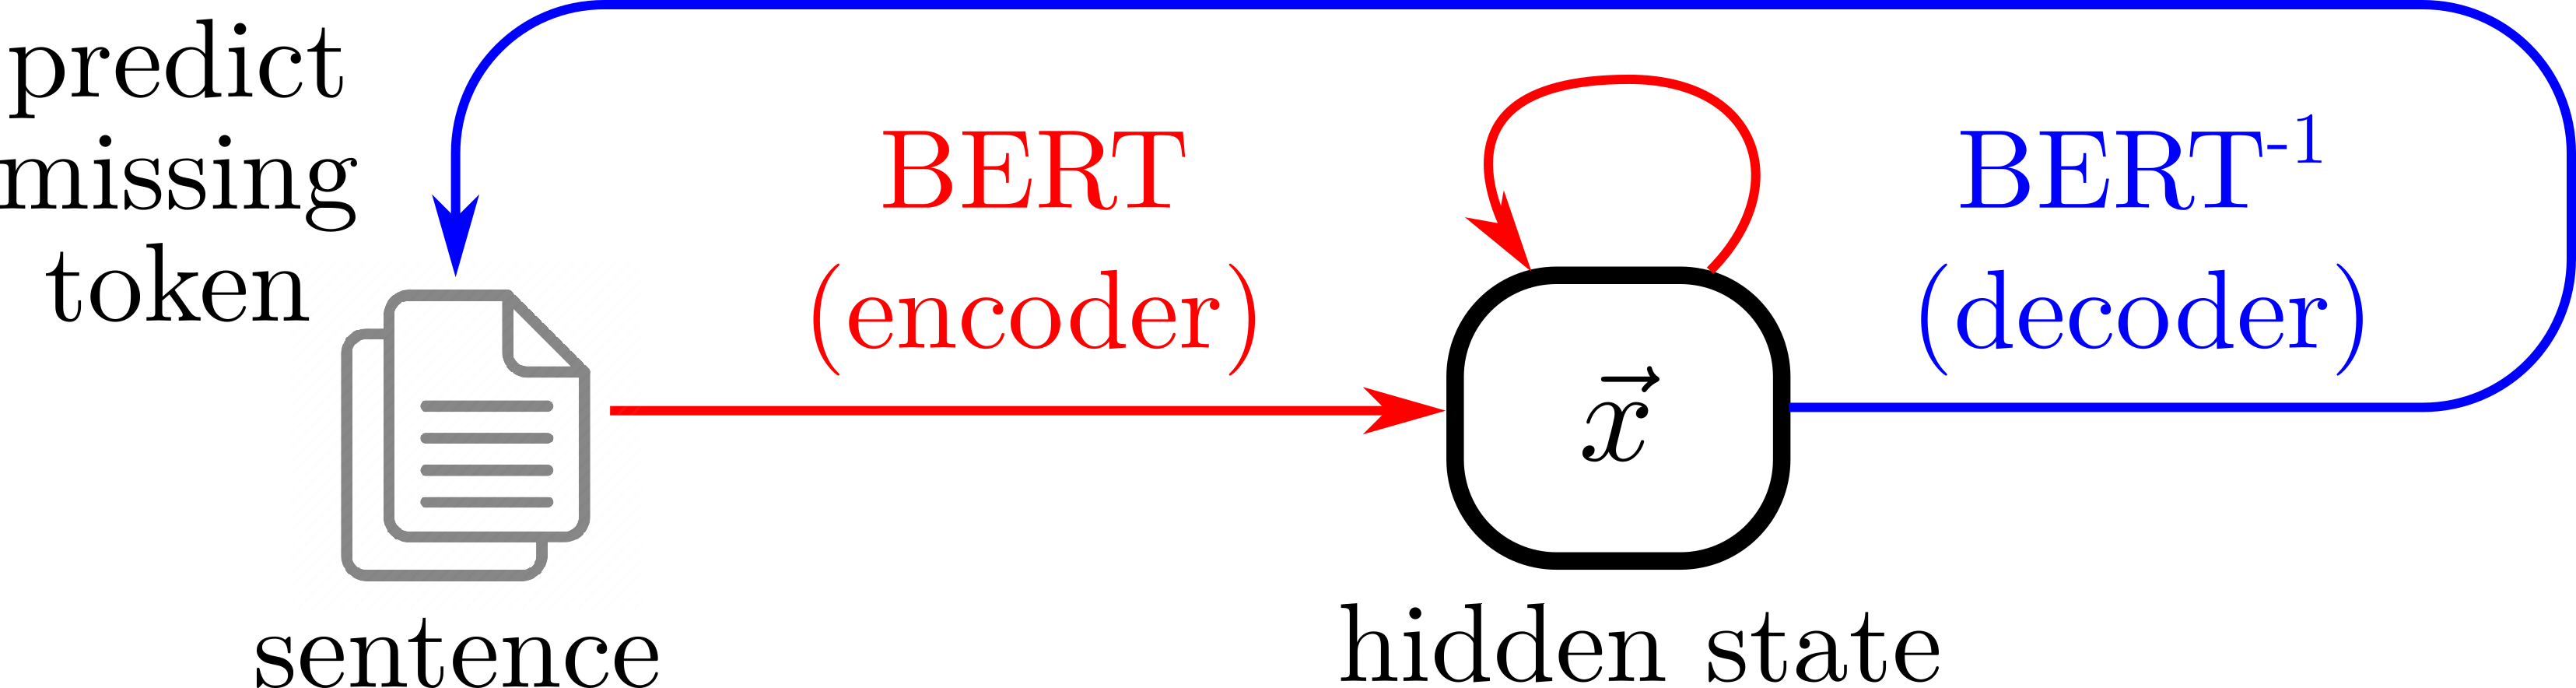
\includegraphics[scale=0.5]{BERT-architecture.png}}}
	\end{equation}
	\cc{换句话说: 隐状态的 representation 压缩了句子的意思,而它可以应用在别的场景下}
	{In other words, the hidden state compresses the meaning of sentences, that can be used in other scenarios}
	
	\item This implies that human-level AI can be \textit{induced} from existing corpora, \cc{而\emp{不需重复 像人类婴儿成长的学习阶段}}
	{without the need to \emp{retrace human infant development}}

	% \item Such corpora can include items such as images, movies with dialogues / subtitles

	\item \cc{这种训练方法是较早的另一篇论文提出,它并不属於 BERT 的内部结构}
	{This training technique came from an earlier paper, unrelated to BERT's internal architecture}
\end{itemize}
\end{frame}

\begin{frame}
\frametitle{\cc{BERT 的内部结构}
	{BERT's internal architecture}}
\cc{其实,BERT 也是混合了很多技巧 发展而成的:}
{BERT results from combining several ideas:}
\begin{itemize}
\item \cc{BERT 基本上是一个 seq-to-seq 的运算过程}
{BERT is basically a seq-to-seq transformation}
\item \cc{Seq-to-seq 问题最初是用 RNN 解决的}
{Seq-to-seq was originally solved by RNNs}
\item \cc{但 RNN 速度较慢,有人提出用 CNN 取代:}
{But RNNs are slow, researchers proposed to replace them with CNNs}
\begin{equation}
\vcenter{\hbox{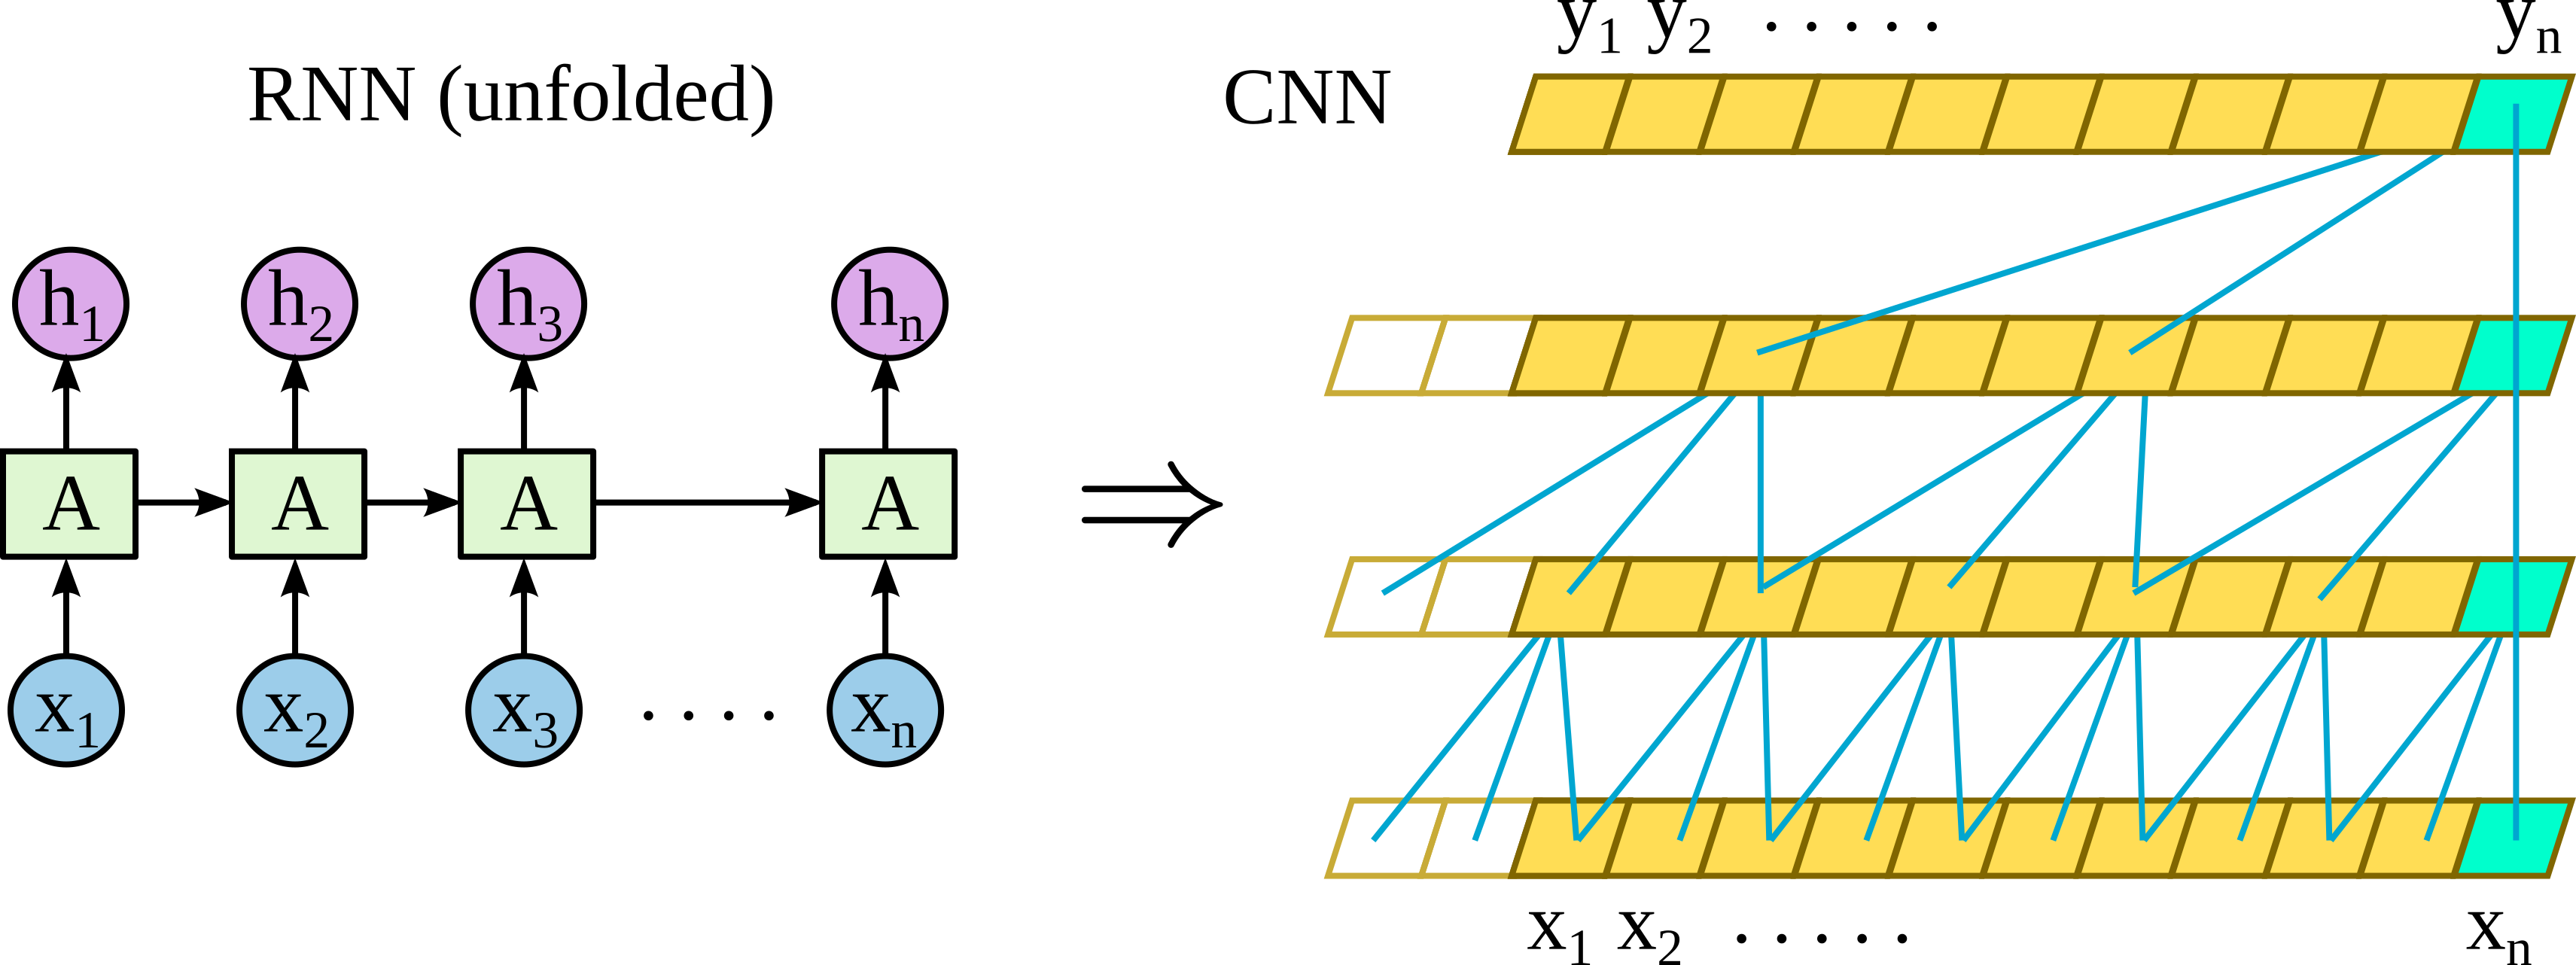
\includegraphics[scale=0.5]{RNN-2-CNN.png}}}
\end{equation}
\item \cc{CNN 加上 attention mechanism 变成 Transformer}
{CNN with \emp{attention mechanism} gives rise to Transformer}
\item \cc{我的想法是重复这个思路,但引入 逻辑的对称性}
{My idea is to incorporate logical symmetry into BERT while following this line of thinking}
\end{itemize}
\end{frame}

\begin{frame}
\frametitle{Symmetry in logic}
\begin{itemize}
	\item \cc{\emp{词语} 组成 \emp{句子},类比於 逻辑中,\emp{概念} 组成 \emp{逻辑命题}}
	{\emp{Words} form \emp{sentences}, analogous to \emp{concepts} forming \emp{propositions} in logic}
	
	\item \cc{抽象地说,逻辑语言 可以看成是一种有 2个运算的 \emp{代数结构}:加法($\wedge$,合并命题,可交换)和 乘法($\cdot$,用作概念合成,不可交换)}
	{From an abstract point of view, logic can be seen as an \emp{algebra} with 2 operations: a non-commutative multiplication ($\cdot$, for composition of concepts) and a commutative addition ($\wedge$, for conjunction of propositions)}

	\item \cc{例如:}{For example:}
	\begin{equation}
	\begin{aligned}
	A &\wedge B & \equiv && B & \wedge A \\
	\mbox{\cc{下雨}{it's raining}} &\wedge \mbox{\cc{失恋}{lovesick}} & \equiv && \mbox{\cc{失恋}{lovesick}} &\wedge \mbox{\cc{下雨}{it's raining}}
	\end{aligned}
	\end{equation}

	\item \cc{Word2Vec 也是革命性的; 由 Word2Vec 演变成 Sentence2Vec 则比较容易,基本上只是 向量的 \emp{合并} (concatenation);  Sentence 对应於 逻辑命题}
	{Word2Vec was also ground-breaking, but it was easy to go from Word2Vec to Sentence2Vec: just concatenate the vectors
	\\ Sentences correspond to propositional logic}

	\item \cc{但 命题的 \emp{集合} 需要用 symmetric NN 处理,因为 集合的元素 是\emp{顺序无关}的}
	{A \emp{set} of propositions requires symmetric NN to process, as elements of the set are \emp{permutation invariant}}

	% \item 假设 全体逻辑命题的空间是 $\mathbb{P}$,则 \emp{命题集合} 的空间是 $2^{\mathbb{P}}$,非常庞大
	
	% \item 如果限制 状态 $\vec{x}$ = working memory 只有 10 个命题,$\vec{x}$ 的空间是 $\mathbb{P}^{10}/\sim$ 其中 $\sim$ 是对称群 $\mathfrak{S}_{10}$ 的等价关系。 换句话说 $ 2^{\mathbb{P}} \cong \coprod_{n=0}^{\infty} \; \mathbb{P}^n / \mathfrak{S}_n $
	
	% \item $\mathbb{P}^n / \mathfrak{S}_n$ 虽然是 $\mathbb{P}^n$ 的商空间,但 $\mathfrak{S}_n$-不变性 很难用神经网络实现
	
	% \definecolor{darkgreen}{rgb}{0.1, 0.7, 0.2}
	% \item 现时 比较可行的办法,是将 状态 $\vec{x}$ 实现成 一个时间上的「轮盘」,每个 ${\color{darkgreen}\bullet}$ 表示一个命题:
	% \begin{equation}
	% \vcenter{\hbox{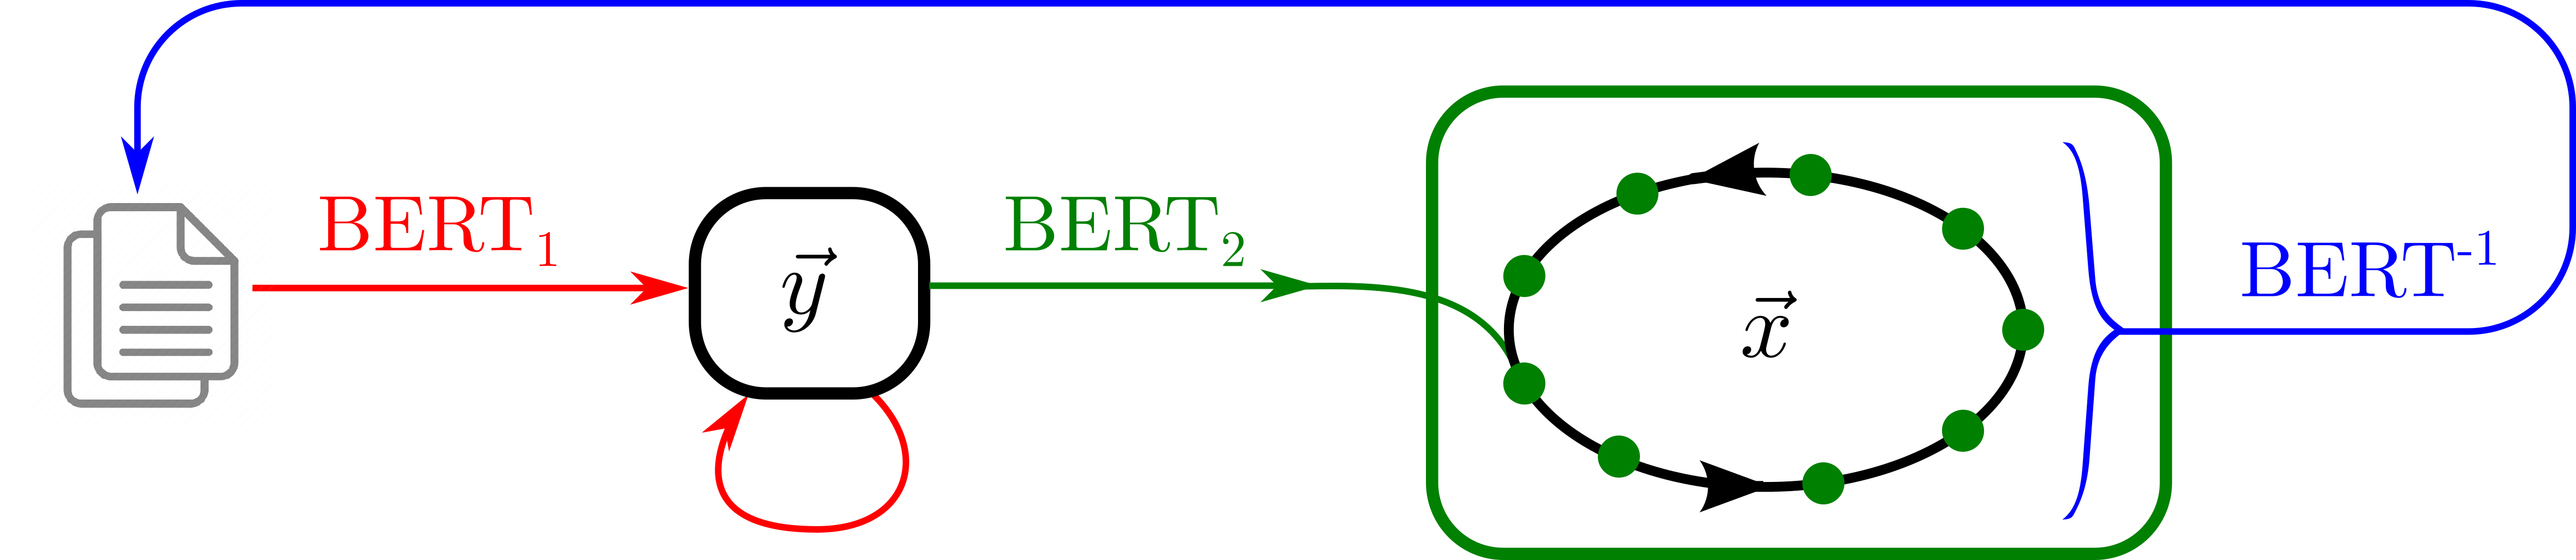
\includegraphics[scale=0.5]{BERT-with-carousel-architecture-1.png}}}
	% \end{equation}
	
	% \item 有趣的是,如果用「轮盘」方法,BERT 的 \emp{注意力机制} 有特殊意义....
\end{itemize}
\end{frame}

\begin{frame}
\frametitle{Symmetric neural network}
\begin{itemize}
	% \item Permutation invariance can be handled by \emp{symmetric} neural networks

	\item \cc{Symmetric NN 问题 已经由 两篇论文解决了: \\ \tab [PointNet 2017] [DeepSets 2017]}
	{The symmetric NN problem has been solved by 2 papers: \\ \tab  [PointNet 2017] and [DeepSets 2017]}

	\item Any symmetric function can be represented by the following form (a special case of the Kolmogorov-Arnold representation of functions):
	\begin{equation}
	\label{symmetric-functions}
	f(x, y, ...) = g(h(x) + h(y) + ... )
	\end{equation}
	\begin{equation}
	\vcenter{\hbox{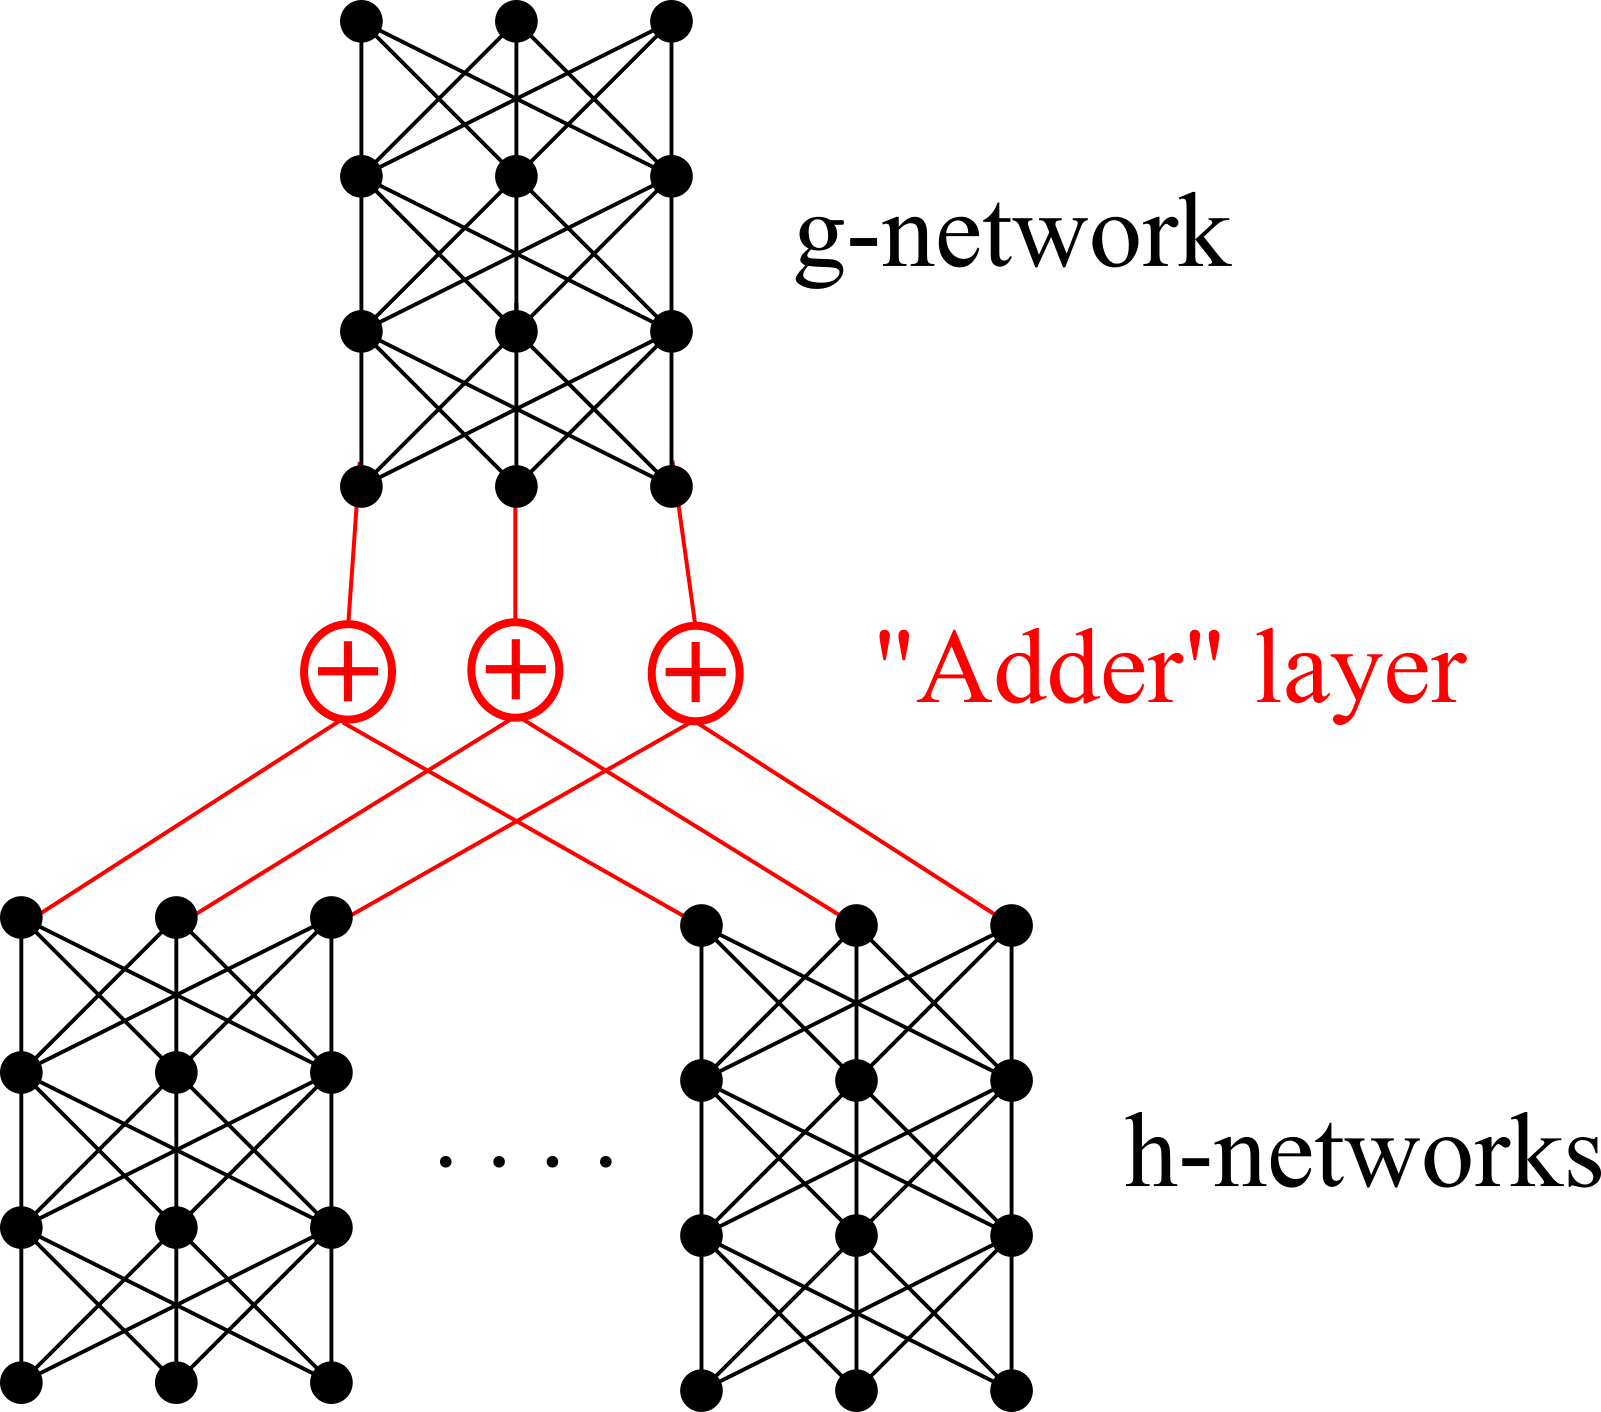
\includegraphics[scale=0.5]{g-and-h-networks.png}}}
	\end{equation}
\end{itemize}
\nocite{Qi2017a}
\nocite{Zaheer2017}
\end{frame}

\begin{frame}
\frametitle{\cc{知识图谱 (knowledge graphs)}{Knowledge graphs}}
\begin{itemize}
	\item \cc{知识图谱 不能直接输入神经网络,它必需分拆成很多 edges,每个 edge 是一个 \emp{关系},也是一个 \emp{逻辑命题} ;也可以说 ``graphs are isomorphic to logic''}
	{One cannot feed a knowledge graph directly into a neural network, as the input must be a vector.  A solution is to break the graph into edges, where each edge is equivalent to a \emp{relation} or \emp{proposition}.  One could say that graphs are isomorphic to logic}
	\begin{equation}
	\vcenter{\hbox{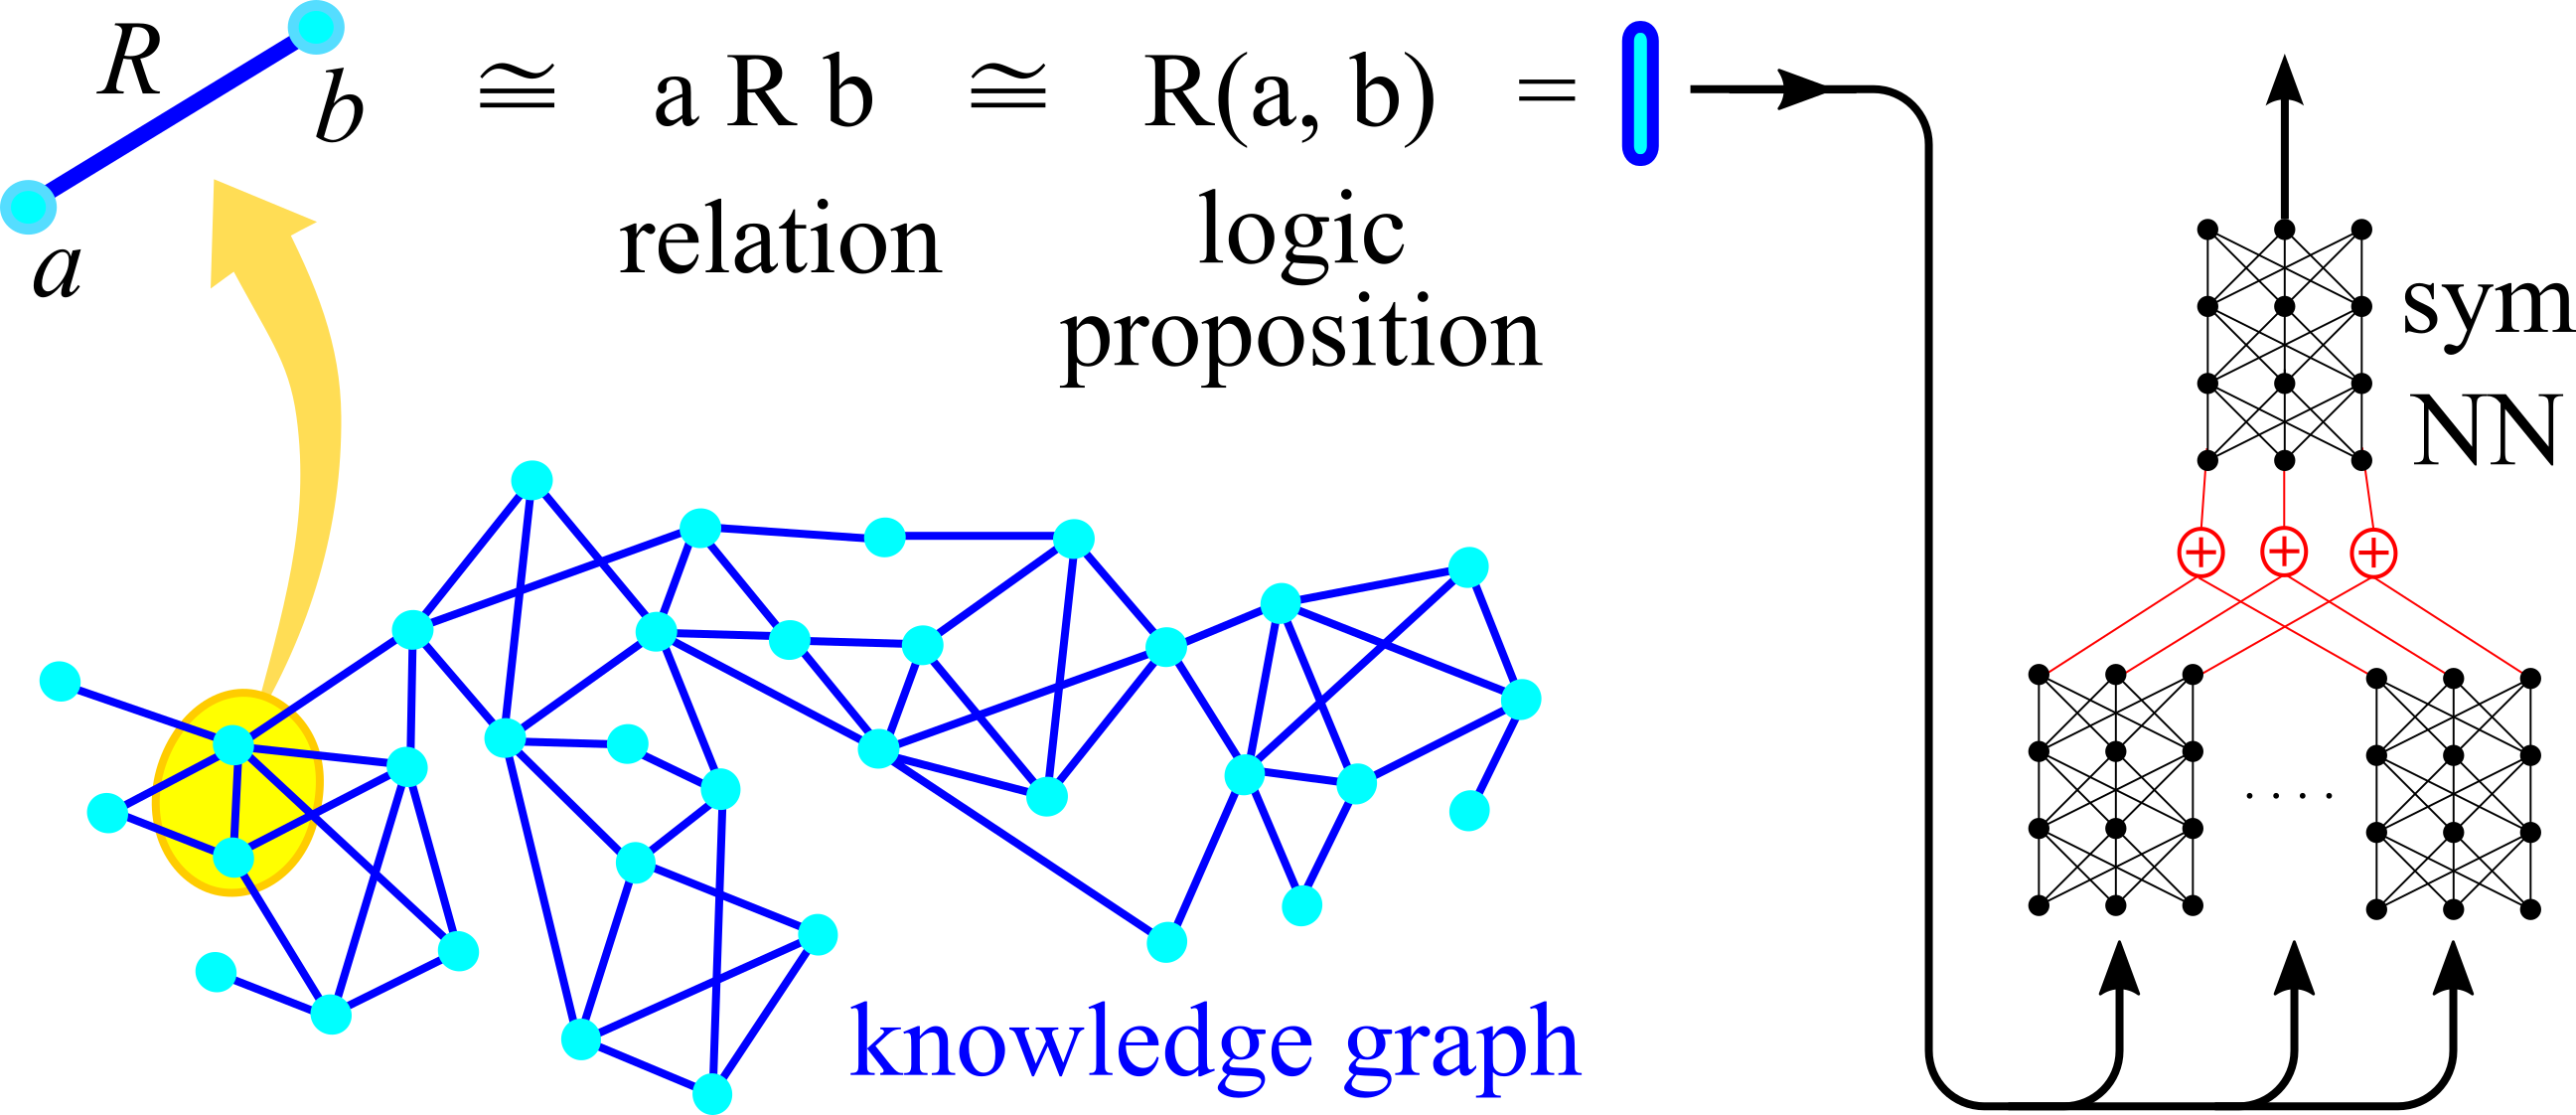
\includegraphics[scale=0.6]{knowledge-graph.png}}}
	\end{equation}
	\item \cc{而这些 edges 似乎必需用 \emp{symmetric} NN 处理,因为它们是 permutation invariant}
	{As edges are invariant under permutations, it seems that we must use symmetric NNs to process them}
	% \item Sym NNs are required to handle \emp{graph-rewriting}, an essential operation on knowledge graphs

	\item \cc{逻辑化 建立了 知识图谱 和 BERT 之间的一道桥梁}
	{Logicalization provides a bridge between BERT and knowledge graphs}
	
	\cc{
	接下来讨论 BERT....}{
	Next we discuss BERT....
	}
	
\end{itemize}
\end{frame}


\begin{frame}
\frametitle{\cc{BERT 的逻辑化}{Logicalization of BERT}}
\begin{itemize}
	\item \cc{可以强逼 BERT 的 隐状态 变成 ``set of propositions'' 的形式,方法是将 对称性 施加在 Encoder 上:}
	{We can force BERT's hidden state to be a set of propositions by imposing permutation symmetry on its Encoder:}
	\begin{equation}
	\vcenter{\hbox{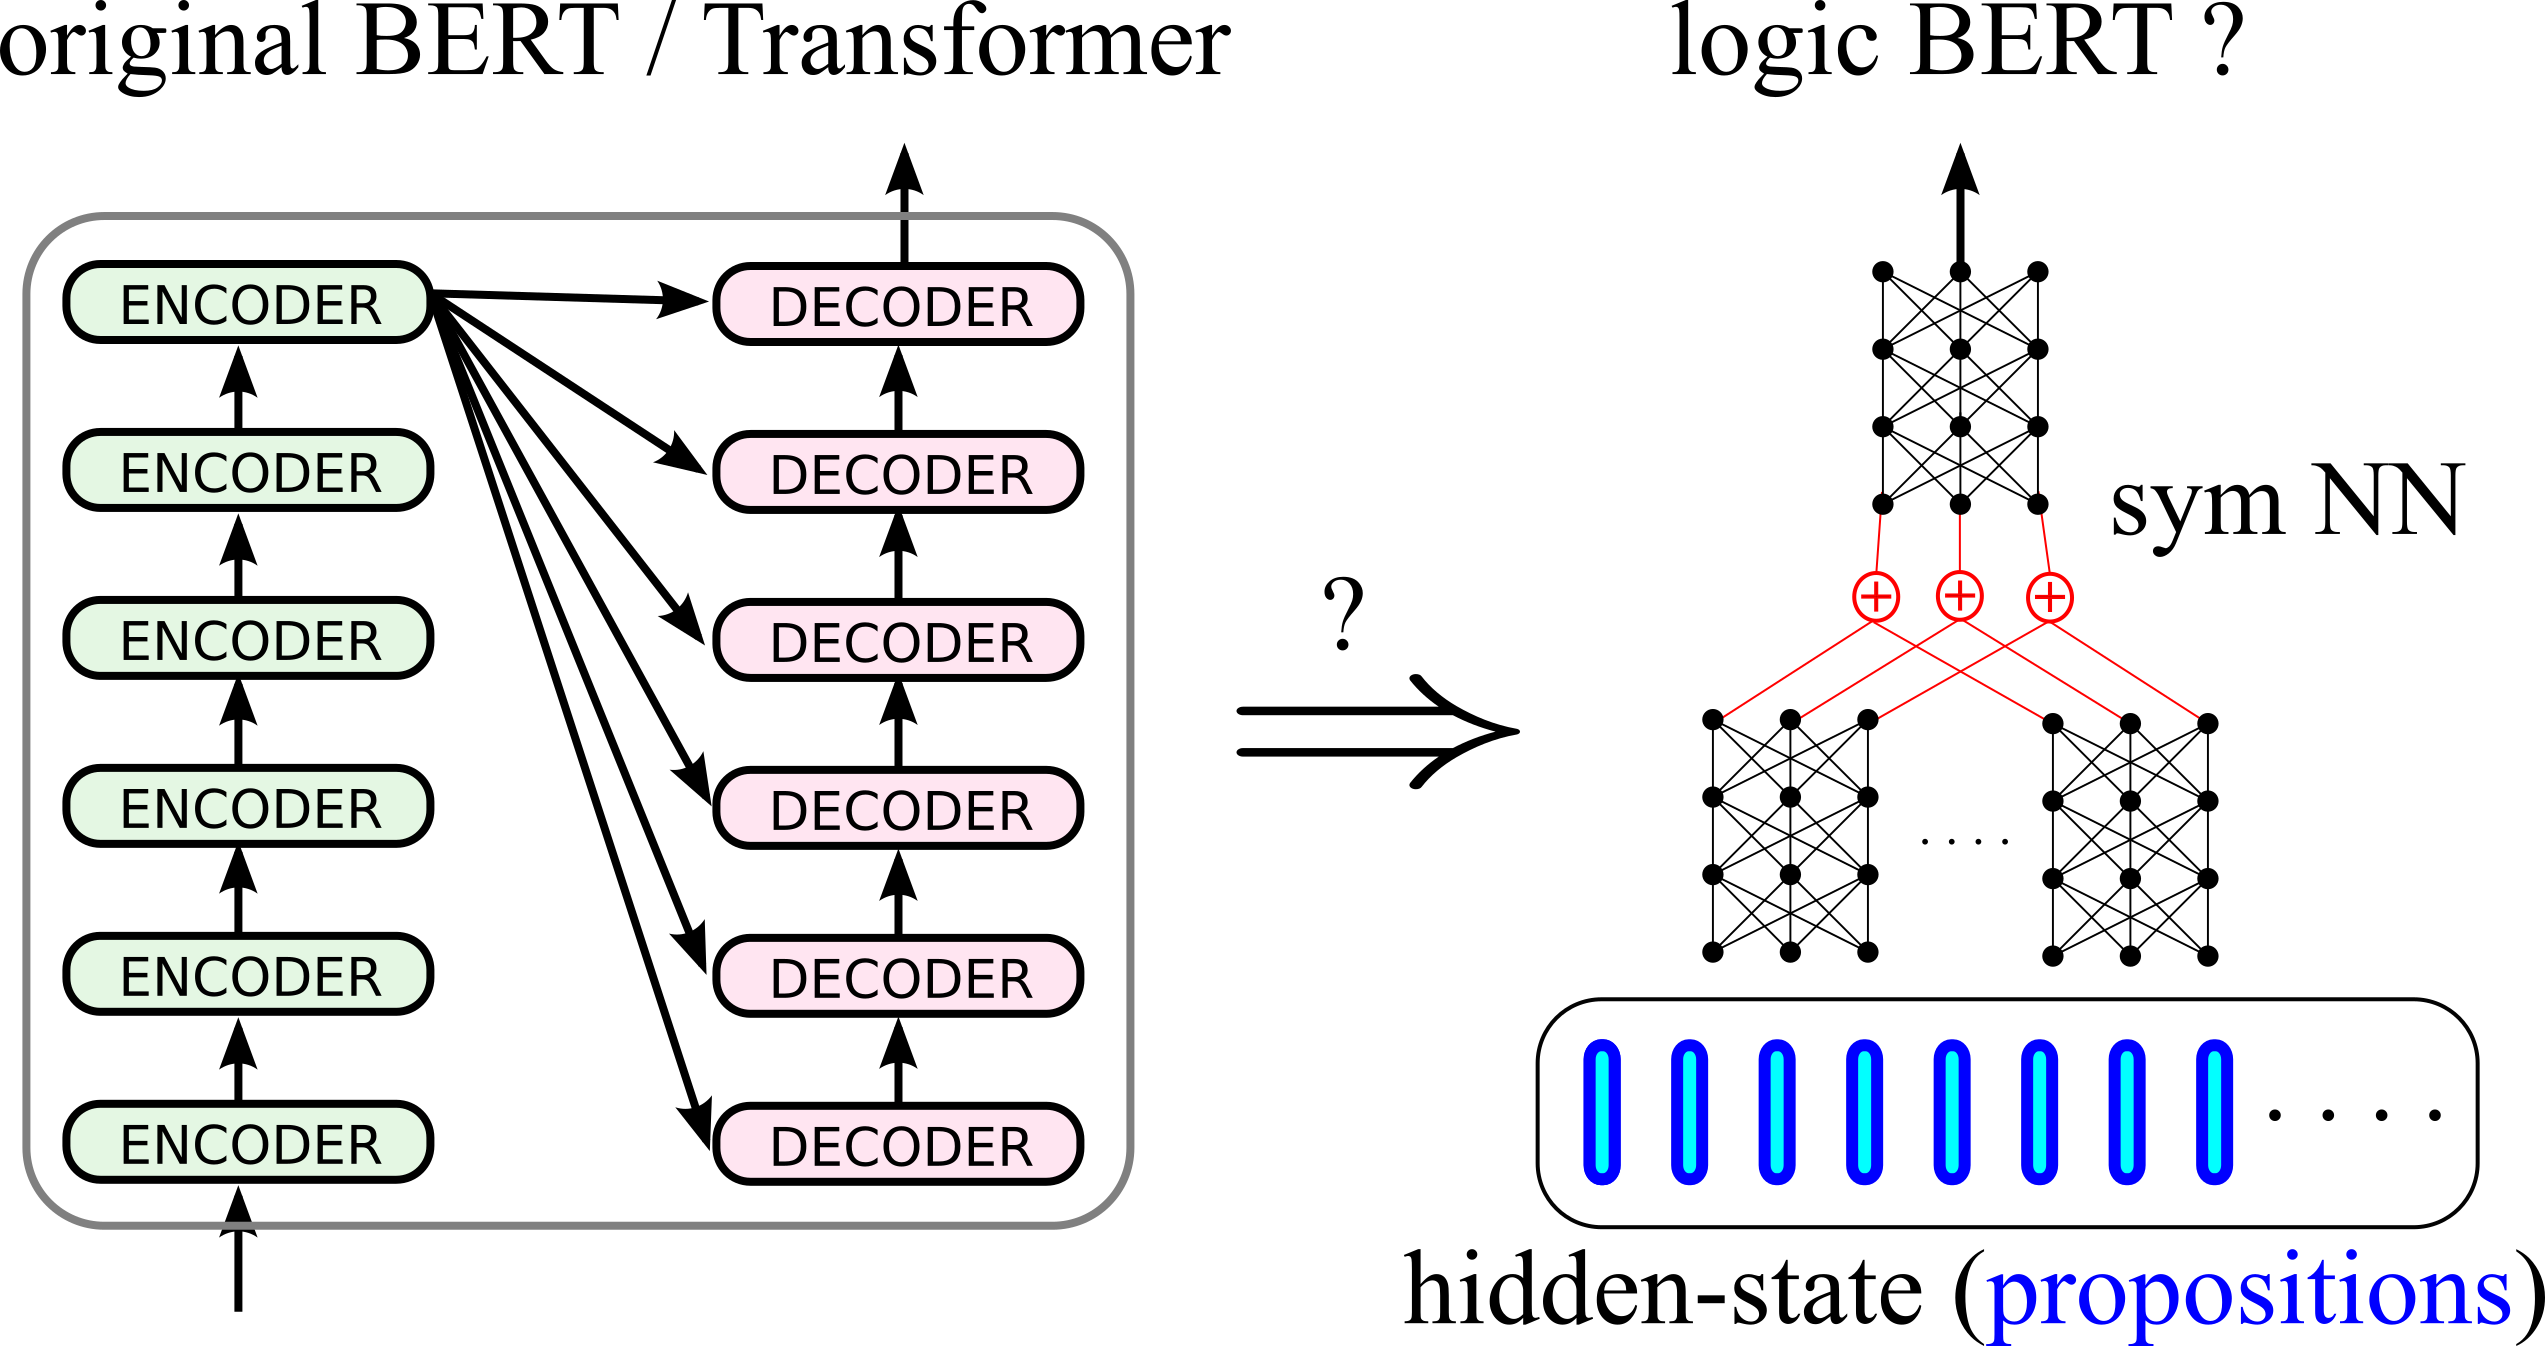
\includegraphics[scale=0.5]{sym-BERT.png}}}
	\end{equation}

	\item \cc{下面会看到,BERT 的「注意力机制 」已经是对称的,它可以做 逻辑推导}
	{Below we'll see that BERT's \emp{attention mechanism} is already symmetric and can perform logic inference}

	% \item \cc{这时,输出对 $\NewSym{proposition.png}$ 的交换不变性 is automatically satisfied by the architecture of the decoder}
	% {Permutation invariance of the $\NewSym{proposition.png}$'s is automatically satisfied by the architecture of the new decoder}

	% \item \cc{旧的 encoder 可以照旧使用,因为它是一个 universal seq-2-seq mapping}
	% {The original \emp{encoder} can be retained, as it is a universal seq-2-seq mapping}
	
	% \item \cc{因为后半部改变了,error propagation 会令 representation 也改变}
	% {The \emp{decoder} imposes symmetry on the hidden state;  Error propagation is expected to cause its representation to change}

	% \item \cc{当然,这个想法有待实验证实 \smiley}
	% {Of course, this remains to be proven by experiment \smiley}
	
	%({\color{red}第一层}似乎可以纳入到{\color{darkgreen}第二层},简化整个模型)
	
	% \item 我发现 最难处理的问题,是在第2层 的状态 $\vec{x}$.  它是一个 逻辑命题 的 \emp{集合},集合中元素有可交换性,亦即 \emp{permutation invariance}.  这看似简单的特性,其实带来很大的麻烦
	
	% \item 如何 standardize 输入空间,使之可以接受任何形式的输入?
	
	% \item BERT 后端的输出可以是 actions,变成一个可以行动的 agent.  如何找大量的资料 训练它?
	
	% \item state $\vec{x}$ 的结构: 用 vector 还是 graph $\cong$ set of logic propositions 比较好? \\
	% 后者有 内在的 逻辑结构,是一种 inductive bias
	
	% \item 现时,所有 知识存在於 BERT 的 weights 里面,可不可以将一部分记忆 转化成 declarative knowledge,储存在 knowledge graph? 这做法有没有好处? 
\end{itemize}
\end{frame}

\begin{frame}[fragile]
\frametitle{\cc{逻辑 与 AI 之间的联系}
{Connection between AI and logic}}
\begin{itemize}
	\item \cc{既然 AI 基於 逻辑,则 AI 与逻辑之间 必然存在 精确 (precise) 的联系}
	{If AI is based on logic, there must exist a \emp{precise} connection between them}

	\item \cc{BERT 似乎是在执行 句子之间的变换,而这些句子是 word embedding 的 concatenation,例如:}
	{BERT seems to be performing some kind of \emp{transformations} between sentences, such sentences are simply compositions of word-embedding vectors:}
	\begin{equation}
	\begin{tikzcd}[column sep = large]
	\mbox{\cc{苏格拉底}{Socrates}} \cdot \mbox{\cc{是}{is}} \cdot \mbox{\cc{人}{human}}
	\arrow[r, "BERT"]
	& \mbox{\cc{苏格拉底}{Socrates}} \cdot \mbox{\cc{会}{is}} \cdot \mbox{\cc{死}{mortal}}
	\end{tikzcd}
	\label{BERT-map}
	\end{equation}
	\cc{这个做法看似很「粗暴」,其实它和 \emp{逻辑式子} 的作用一样:}
	{While this may seem crude, it is effectively the same as a logic formula:}
	\begin{equation}
	\forall x. \; \mbox{Human}(x) \rightarrow \mbox{Mortal}(x)
	\end{equation}
	\cc{而这式子,根据 Curry-Howard 对应,就是 (\ref{BERT-map}) 的函数映射!}
	{Surprisingly, by the Curry-Howard correspondence, this formula corresponds to the mapping (\ref{BERT-map}) above!}

	% \item 这些映射的对象,是形如 ``$a \in A$'' 这样的物体,它们有 predicates 的几何/拓扑结构,但我们现时未做到这一步,暂时只引入了 commutativity
	
	\begin{comment}
	\item 集合元素 $a$ 是 $\exists x. P(x)$ 的证明,例如 Socrates 是 $\exists x. \mbox{mortal}(x)$ 的证明
	\item 当 神经网络 \emp{调教} 某些元素的 映射 (mapping) 时,它同时在学习某个逻辑的 formula;  换句话说,逻辑 是几何空间中的映射
	\item 逻辑的 谓词 (predicates) 是在 基底元素空间上的一个 \emp{纤维丛结构} (fibration) :
	\begin{equation}
	\vcenter{\hbox{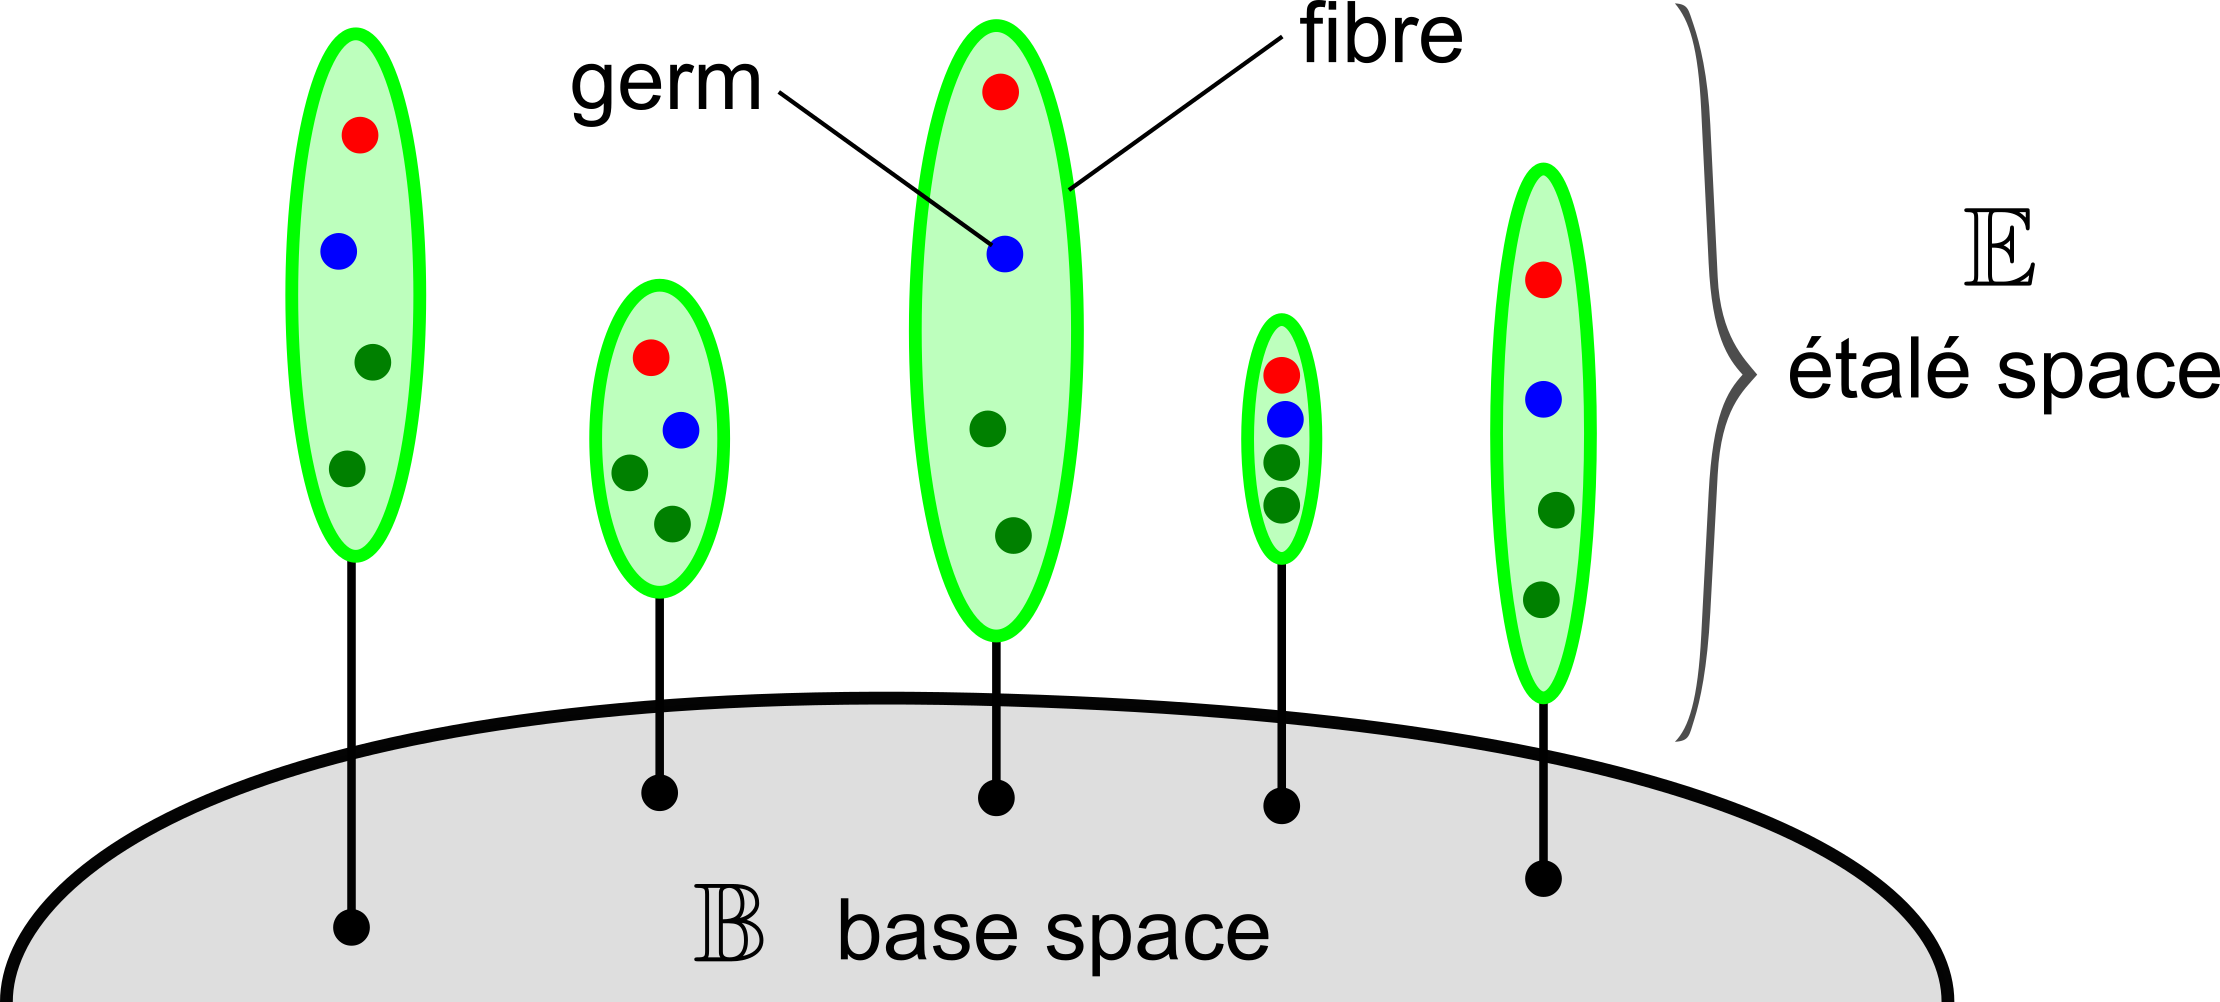
\includegraphics[scale=0.5]{etale-space.png}}}
	\end{equation}
	\end{comment}
	
	% \item 从 几何/拓扑 ``借'' 来的概念,演变成 topos 理论、HoTT 等
	
	% \item 这些漂亮的理论 不是无用的; 有需要时,可以從 邏輯 那邊借來更多的結構
	
	\item \cc{我会在另一辑 slides 里 简介一下这些理论; 可以说,逻辑的 几何结构 是「永恒」的,它可以指示 AI 的 长远发展}
	{In another set of slides we shall explore this connection.  One could say the mathematical structure of logic is ``eternal'';  It will provide guidance for the long-term development of AI}
	
	% \item $H(a)$ is a type.
	% \item $H$ is a prodicate type.
	% \item The proof of $H(a)$ may be the tuple $(a, H)$ or $a \in H$
\end{itemize}
\end{frame}


\begin{frame}
\frametitle{\cc{Attention 是什么?}{What is attention?}}
\begin{itemize}
\item \cc{注意力 最初起源於 Seq2seq,后来 BERT 引入 self-attention}
{Attention originated with Seq2seq, then BERT introduced self-attention}

\item \cc{Attention 的本质就是 \emp{加权},权值 可以反映 模型 \emp{关注}的点}
{The essence of attention is \emp{weighing}}

\item For each input, attention weighs the \emp{relevance} of every other input and draws information from them accordingly to produce the output

\item \cc{在 BERT 里,attention 是一种 \emp{words} 之间的关系:}
{In BERT, attention is a relation among \emp{words} in a sentence:}
\begin{equation}
\vcenter{\hbox{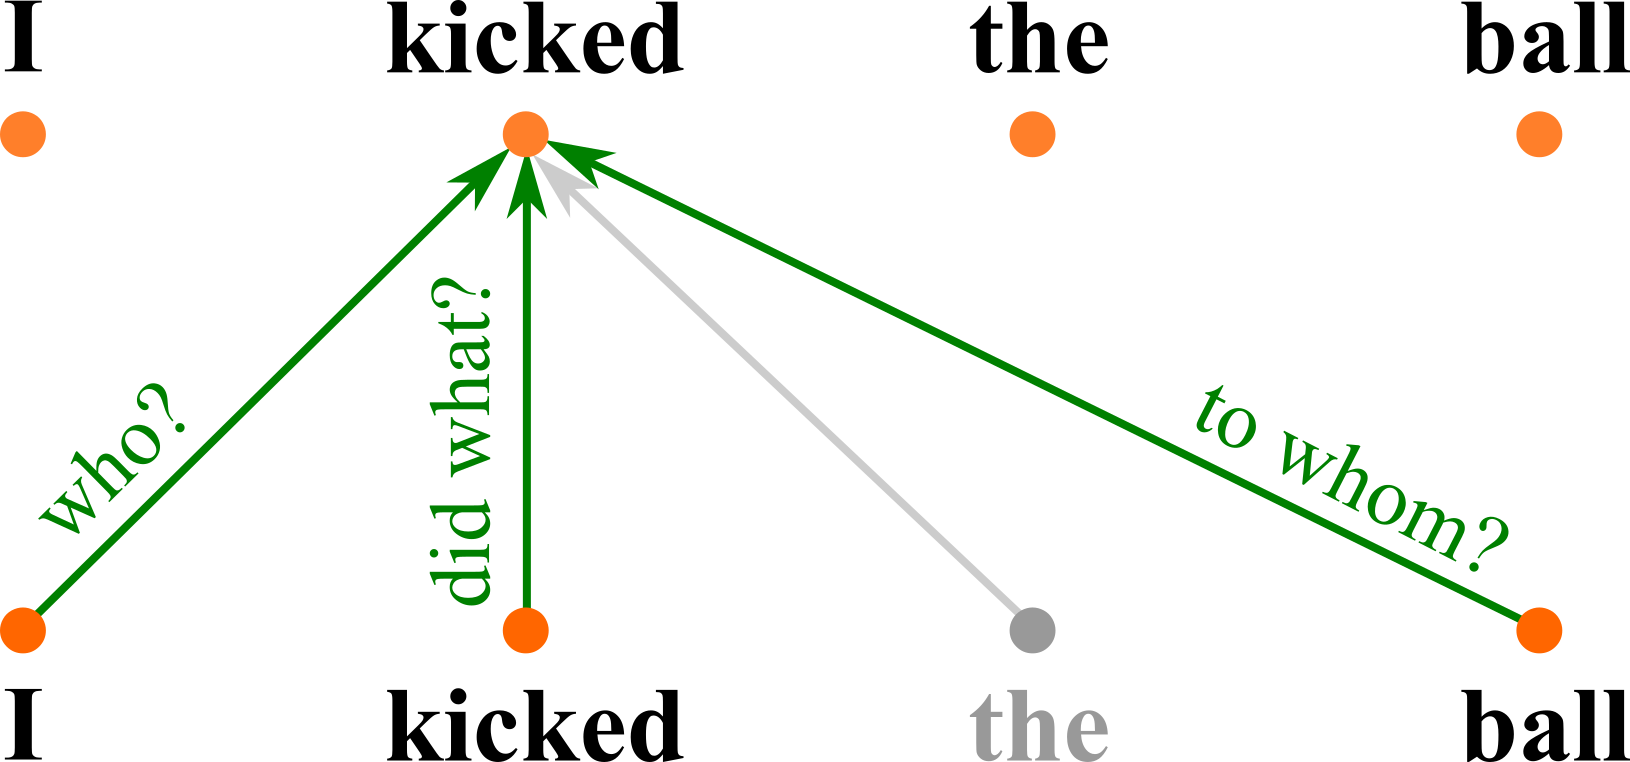
\includegraphics[scale=0.5]{attention-among-words.png}}}
\end{equation}

\item \cc{但,从逻辑的角度看,word $\ne$ 命题}
{From a logic point of view, words $\ne$ propositions}

\item \cc{在逻辑学上,必需分清 命题\emp{内部} 与 命题\emp{之间} 这两个层次,非常关键!}
{In logic, the distinction between sub-propositional and propositional levels is of crucial importance!}

%\item 在 Seq2seq 中,编码器 (encoder) 由下式给出,它将输入的词语 $x_i$ 转化成 一连串的 隐状态 $h_i$:
%\begin{equation}
%h_t = \mbox{RNN}_{encode}(x_t, h_{t-1})
%\end{equation}

%\item 这些 $h_i$ 可以综合成单一个 隐状态 $c = q(h_1, ..., h_n)$. 

%\item 这个 $c$ 被「寄予厚望」,它浓缩了整个句子的意义

%\item 解码器 的结构类似,它的隐状态是 $s_t$,输出 $y_t$:
%\begin{equation}
%s_t = \mbox{RNN}_{decode}(y_t, s_{t-1}, c_t)
%\end{equation}

%\item 注意最后的 $c_t$ 依赖时间,它是隐状态 $h_j$ 的 \emp{加权平均}:
%\begin{equation}
%c_i = \sum_j \alpha_{ij} h_j
%\end{equation}

%\item 其中 $\alpha_{ij}$ 量度 输入/输出 的隐状态之间的 \emp{相似度},取其最大值:
%\begin{equation}
%\alpha_{ij} = \mbox{softmax} \{ \langle s_i, h_j \rangle \}
%\end{equation}
%换句话说,$\alpha_{ij}$ \emp{选择} 最接近 $h_j$ 的 $s_i$
\end{itemize}
\end{frame}

\begin{frame}
\frametitle{\cc{谓词 (predicates) vs 命题 (propositions)}
	{Predicates vs propositions}}
\begin{itemize}
\item \cc{``Predicate'' 来自拉丁文「断言」的意思}
{The word ``predicate'' comes from Latin ``to declare''}

\item \cc{逻辑里,predicate 代表一个 没有主体/客体 的断言,换句话说,是一个有「洞」的命题}
{In logic, a predicate is a declaration without a subject or object;  In other words, it is a proposition with ``holes''}
	
\item \cc{\emp{命题} = \emp{谓词} (predicate) + \emp{主体/客体}(统称 objects)}
{\emp{Proposition} = \emp{predicate} + \emp{objects}}

\item \cc{例如:}{Eg:} Human(John), Loves(John, Mary)

% \item 命题\emp{内部} 的结构,即 predicate-level 结构,命题\emp{之间} 的结构,即 命题逻辑

\item \cc{从逻辑的角度看,attention 的输出可以看成是 predicate 和 objects 的\emp{结合}:}
{From the logic point of view, the output of attention is the \emp{fusion} of a predicate with its objects:}
\begin{equation}
\vcenter{\hbox{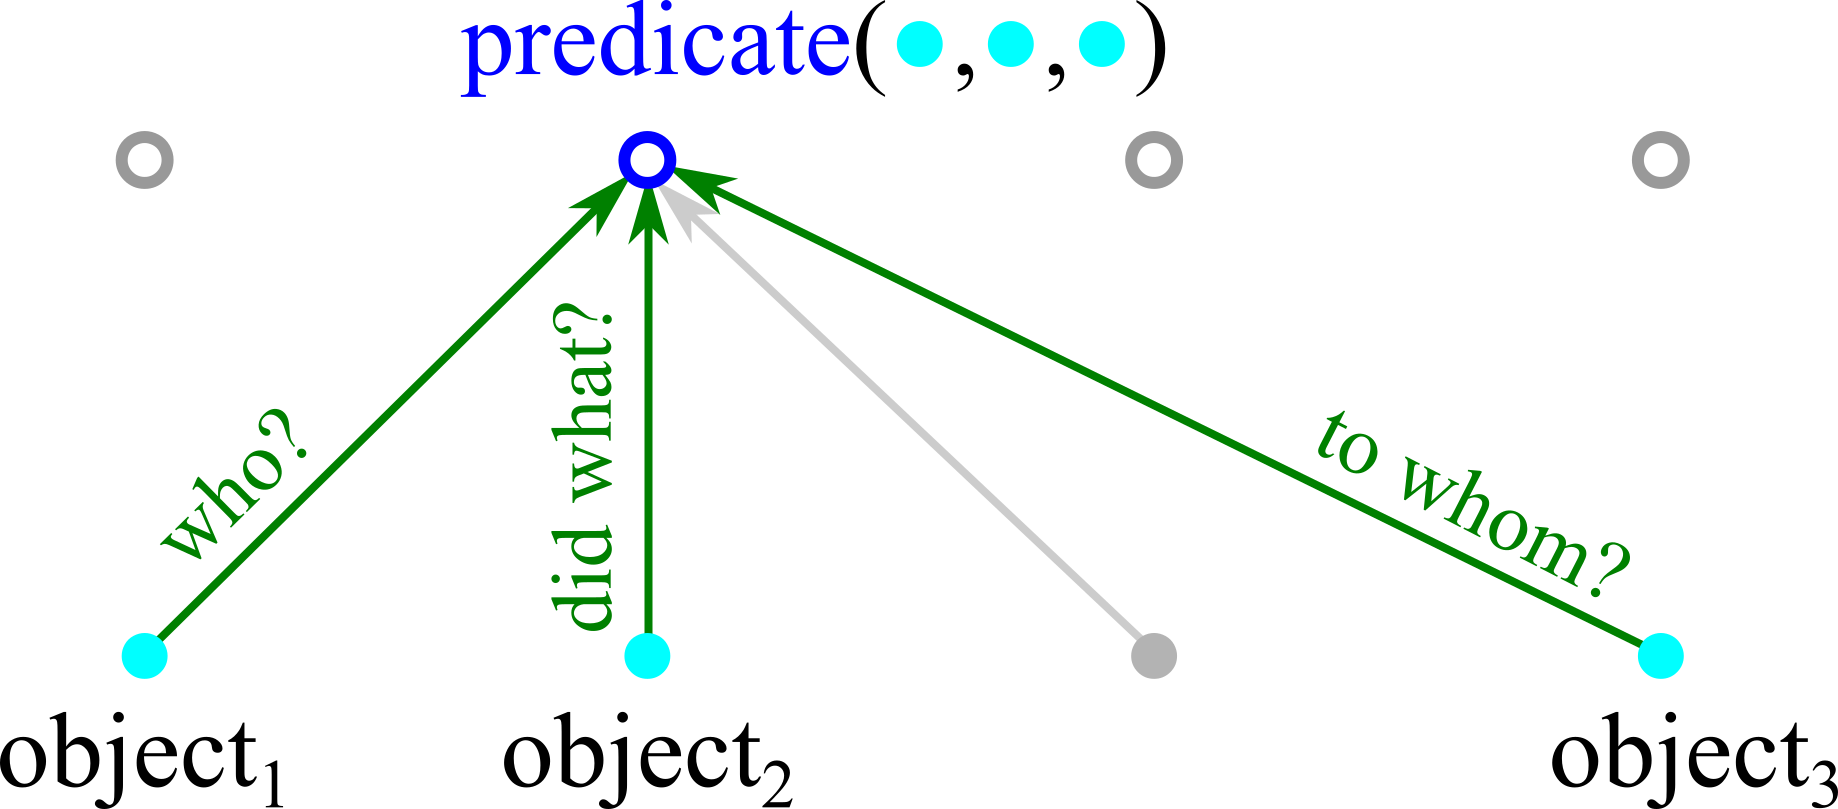
\includegraphics[scale=0.5]{attention-as-predicate.png}}}
\end{equation}

\item \cc{形象地说:}{Or figuratively:}
\begin{equation}
\begin{aligned}
\mbox{predicate} & + \mbox{objects} &&= \mbox{proposition} \\
\NewSym{predicate.png} &+ \NewSym{object.png} \; \NewSym{object.png} \; \NewSym{object.png} \; .... &&= \NewSym{proposition.png}
\end{aligned}
\end{equation}
\end{itemize}
\end{frame}

\begin{comment}
\begin{frame}
\frametitle{Attention 给逻辑 AI 的启发}
我这样理解 attention:
\begin{itemize}
\item 例如,翻译时,输入/输出句子中「动词」的位置可以是不同的

\item 当 解码器需要一个「动词」时,它的隐状态 $s_t$ 含有「动词」的意思

\item Attention 机制 找出最接近「动词」的 编码器的隐状态 (可以 $\ge 1$ 个)$\sum h_j$,交给 解码器,这是一种 \emp{information retrieval}

\item 例如,将 $M$ 件东西 映射 到 $N$ 件东西,可以有 $N^M$ 个 mappings,这是非常庞大的空间。 但如果这些物件有 \emp{类别},而\underline{同类只映射到同类},则可以用 attention 简化 mappings

\item 所以 attention 是一种 inductive bias,它大大地缩小 mapping 空间

\item 在逻辑的场景下,需要的 mapping 是 $f: \mbox{命题集合} \rightarrow \mbox{命题}$
\begin{equation}
\vcenter{\hbox{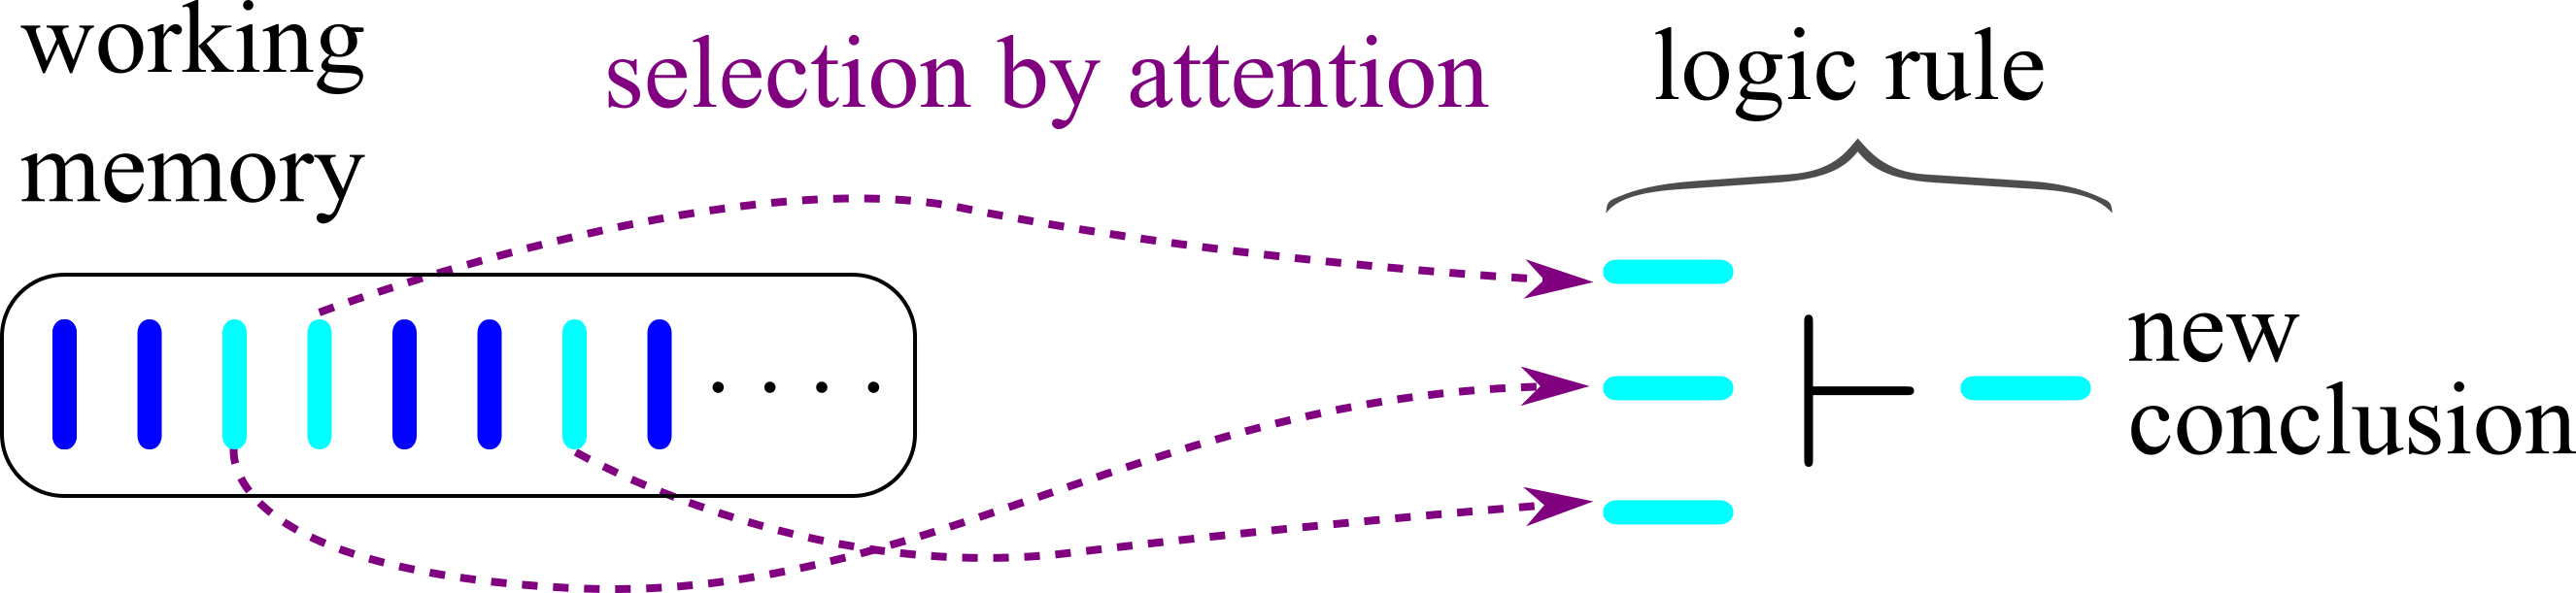
\includegraphics[scale=0.5]{attention-in-logic.png}}}
\end{equation}

\end{itemize}
\end{frame}
\end{comment}

\begin{frame}
\frametitle{``Attention is all you need'' ?}
% \frametitle{\cc{Attention 在命题之间的作用}
%	{Attention at the propositional level}}
\begin{itemize}
\item \cc{类似地,\emp{高层}的 attention 可以处理 \emp{命题之间} 的关系}
{Analogously, attention on higher levels process relations \emp{among} propositions}

% \item \cc{由词语构成句子/命题,通常有少数的 syntax 法则,例如}
% {When forming sentences from words, there are relatively few syntactic patterns, such as:}
% \\ \tab subject $\cdot$ verb $\cdot$ object

% \item \cc{但由命题构成结论,并没有 \textit{a priori} 的规则; 逻辑上有关联的东西 未必是相似的}
% {But there are no \textit{a priori} patterns for forming deductions from propositions;  Logically related things need not be similar}

% \item \cc{例如: 尿急 $\wedge$ 不在厕所 $\Rightarrow$ 忍著; 但「尿」和「厕所」是 \emp{后天} 学习的关系}
% {Eg: need to pee $\wedge$ not in toilet $\Rightarrow$ hold it \\ But ``pee'' and ``in toilet'' is learned \textit{a posteriori}}

\item \cc{我们希望 attention 做到的是 \emp{选择}有关联的命题,去做逻辑推导:}
{We wish for attention to \emp{select} propositions that are relevant for deduction:}
\begin{equation}
\vcenter{\hbox{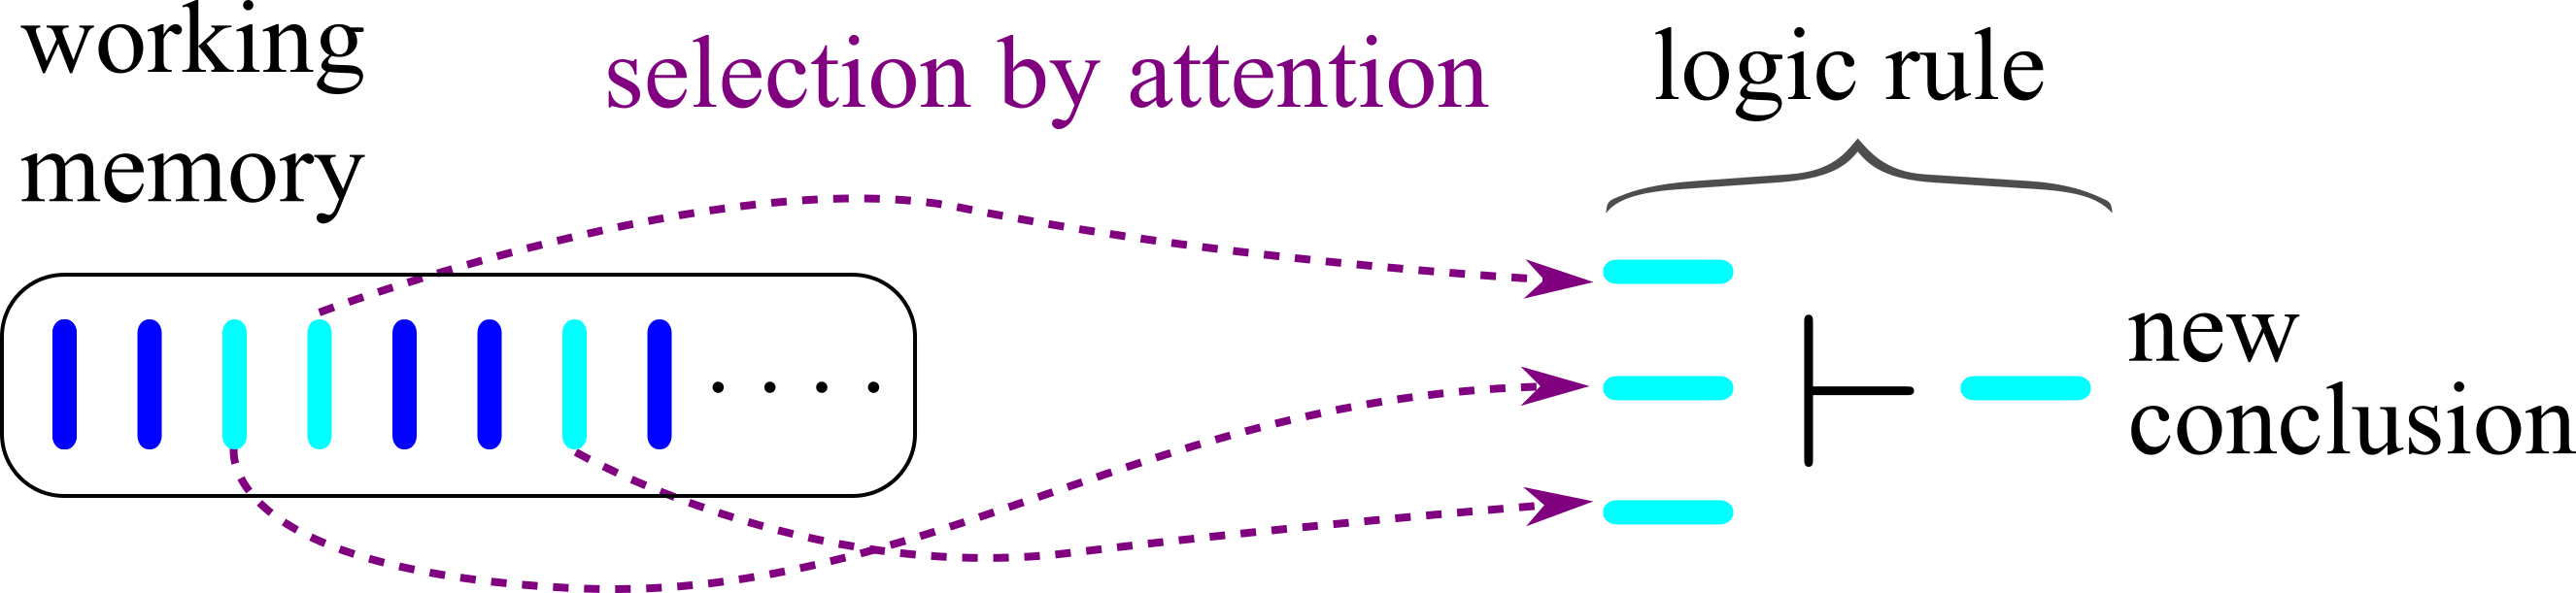
\includegraphics[scale=0.5]{attention-in-logic.png}}}
\end{equation}

\item \cc{但从 $N$ 个命题中选择 $K$ 个,可以有 $N \choose K$ 个子集,是 exponential 的}
{But to choose $K$ propositions from a set of $N$, there would be $N \choose K$ subsets, an \emp{exponential} number}

\item \cc{BERT 的做法是: 每次只输出 $N$ 个命题,而前提的 ``support'' 也是上一层的 全部 $N$ 个命题,每个前提的「影响力」由 matrix 权重决定}
{BERT's way is to output only $N$ propositions per each layer, each proposition is ``supported'' by all $N$ propositions in the previous layer;  The influence of premises are weighted by a matrix}

\item \cc{根据 Curry-Howard isomorphism,BERT 的映射  其实对应於某种 \emp{另类的逻辑}(BERT 的设计者可能没有意识到这点),这种逻辑的好处是运行\emp{非常快}}
{By the Curry-Howard isomorphism, BERT's mapping corresponds to some kind of \emp{alternative logic} (BERT's creators may not have recognized this), which has \emp{very fast} execution}

\item \cc{BERT 的逻辑 看似有局限,但这种表面的局限未必阻止它是 universal 的逻辑}
{BERT's logic seems highly restricted, but the superficial restrictions may not prevent it from being a \emp{universal} logic}

\item \cc{关键是在 速度 与 逻辑的 expressive power 之间 找到平衡}
{The key is to find a balance between speed and expressive power of the logic}
\end{itemize}
\end{frame}

\begin{frame}[plain]
\begin{itemize}
	\item \cc{ 
	最简单的 attention 公式是(其中 $Q, K, V$ = query, key, value 矩阵):}{
	The simplest attention formula is: (where $Q, K, V$ = query, key, and value matrices)
	}
	
	\begin{equation}
	\label{attention-formula}
	\vect{y}_j = \sum_i \langle Q {\color{red}\vect{x}_j} , K \vect{x}_i \rangle V \vect{x}_i
	\end{equation}
	\cc{
	({\color{red}红色} 代表注意力的 focus) 这对应於一个逻辑式子:}{
	({\color{red}red} indicates the focus of attention)  This corresponds to a logic formula:
	}
	
	\begin{equation}
	\vcenter{\hbox{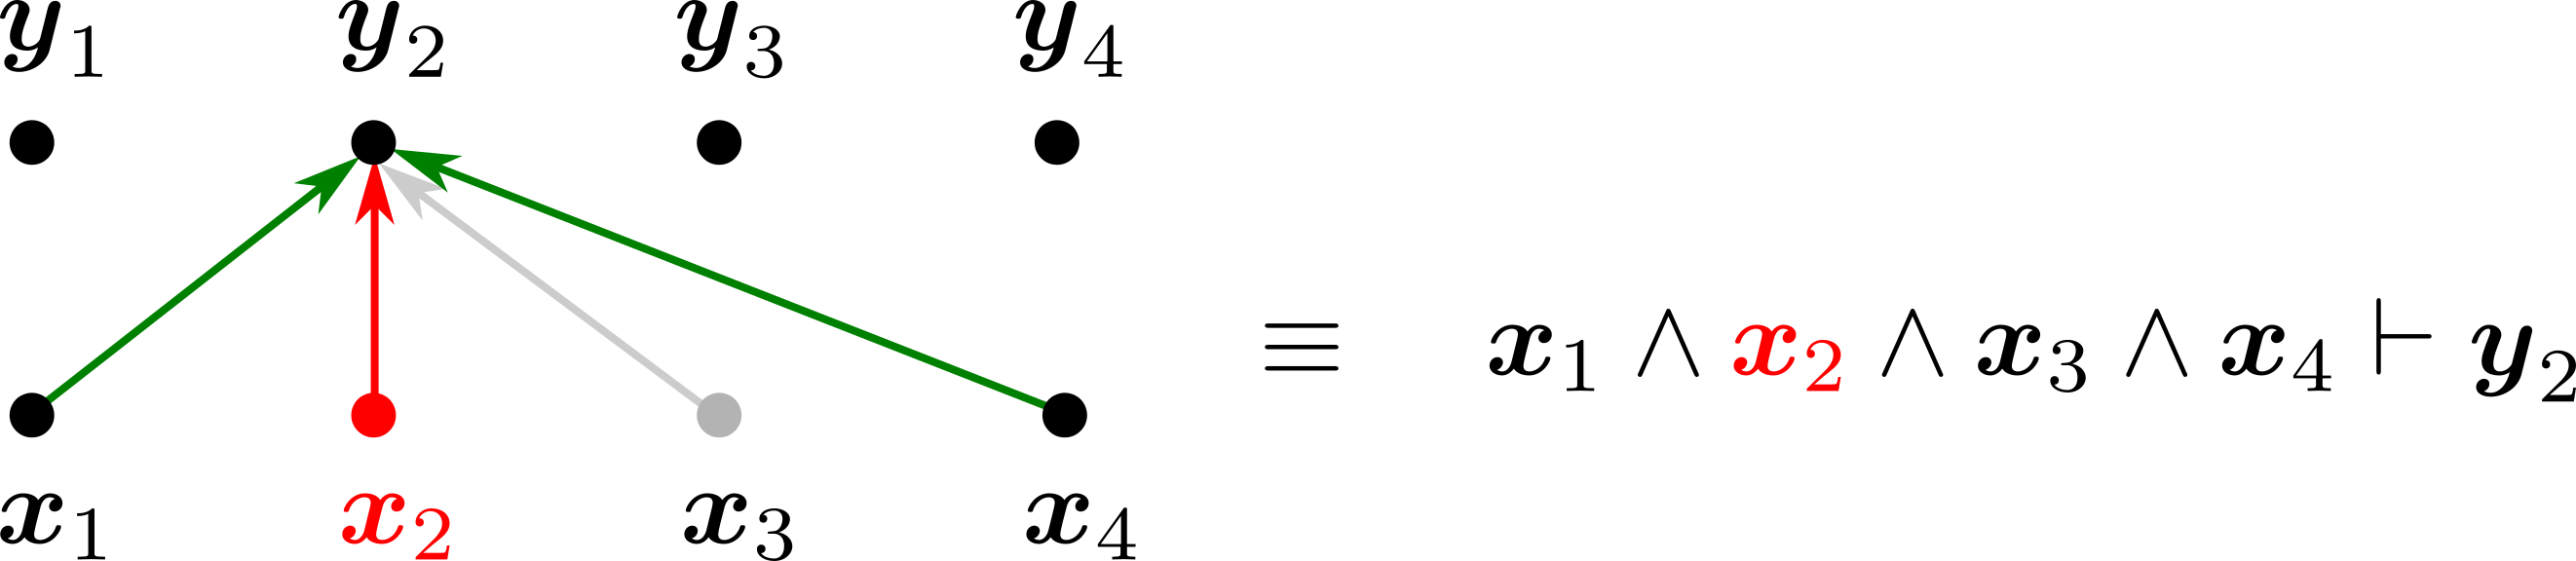
\includegraphics[scale=0.5]{attention-as-propositional-logic.png}}}
	\end{equation}
	\cc{
	亦即是说: $\vect{y}_j$ 是由 $\vect{x}_1, ..., \vect{x}_n$ 得出的逻辑结论 with focus on ${\color{red}\vect{x}_j}$}{
	In other words: $\vect{y}_j$ is the logic conclusion deduced from $\vect{x}_1, ..., \vect{x}_n$ with focus on ${\color{red}\vect{x}_j}$
	}

	\item \cc{
	所谓 ``focus'' 并不是 逻辑概念,它只是 BERT 加速的 heuristic}{
	``Focus'' is not a logical concept;  it is just a speed-up heuristic of BERT
	}

	\item \cc{
	容易看到,attention 对於 $\vect{x}_1, ..., \vect{x}_n$ 是 \emp{交换不变}的 (equivariant),这表示 每层 attention 的输出是一些 \emp{逻辑命题},和我的理论相符}{
	Easy to see that attention is permutation \emp{equivariant} over $\vect{x}_1, ..., \vect{x}_n$, implying that its output are \emp{logic propositions}, consistent with my theory
	}
	
	\item \cc{
	\emp{Multi-head} attention 亦有一个很好的逻辑解释: 即使 focus = ${\color{red}\vect{x}_j}$,亦有其他不同的前提,可以导致不同的结论,例如:}{
	We can also give a logical interpretation to \emp{multi-head} attention:  given the focus ${\color{red}\vect{x}_j}$, there could be other premises leading to different conclusions:
	}
	\begin{equation}
	{\color{red}\vect{x}_1} \wedge \vect{x}_2 \wedge \vect{x}_3 \vdash \vect{y}_1
	\quad , \quad
	{\color{red}\vect{x}_1} \wedge \vect{x}_4 \wedge \vect{x}_5 \vdash \vect{y}_2
	\end{equation}
\end{itemize}
\end{frame}

\begin{frame}
\frametitle{\cc{BERT 为什么成功?}{Why is BERT so successful?}}
\begin{itemize}
	\item \cc{6 层的 BERT 有 $512 \times 6 = 3072$ 个 head,如果 $8\times$ multi-head 则有 24576 个}
	{The 6-layer BERT has $512 \times 6 = 3072$ heads, or 24576 with $8\times$ multi-head attention}
	% 如果每个 head 对应一条 逻辑 formula,这是很少的数目,为什么如此少量的 logic rules 能做到非常成功的效果?		
	% If each head corresponds to 1 logic formula, this is a rather small number.  How could few logic rules perform so successfully?
	
	\item Each head does not simply correspond to 1 formula in conventional logic, may require further in-depth analysis....

	\item \cc{
	我的猜测是: BERT 的高层 representation 是一些有 ``high-level'' 意义的命题,就像在视觉中,高层特征 代表一些复杂的物体}{
	My guess is that the representation in BERT's higher layers are ``high-level'' propositions similar to the high-level features that represent complex objects in machine vision.
	}
	
	\item The embedding of high-level propositions in vector space may be ``semantically dense'', meaning that slight changes in the vector position may convey many different meanings
	
	\item \cc{
	由於 logic rules 是以 6 层的 hierarchy 组织而成,这結構具有 ``\emp{deep learning}'' 的特性}{
	Because logic rules are organized in 6 layers of \emp{hierarchy}, this structure has the ``deep learning'' property
	}
\end{itemize}
\end{frame}

\begin{frame}
\frametitle{\cc{}{An improvement of BERT}}
\begin{itemize}
	\item The BERT attention formula (\ref{attention-formula}) has some unnecessary restrictions, where generally we just need a symmetric function in the $\vect{x}_i$'s
	
	\item The general form of symmetric functions is given by (\ref{symmetric-functions})
	
	\item Immitating BERT, we introduce a ``focus'' of attention on ${\color{red}\vect{x}_j}$:
	\begin{equation}
	\vect{y}_j = g( \; h({\color{red}\vect{x}_j}, \vect{x}_1) + .... + h({\color{red}\vect{x}_j}, \vect{x}_n) \; )
	\end{equation}
	this preserves \emp{equivariance}
	
	\item We can use this function to replace the entire BERT Encoder:
	\begin{equation}
	\vcenter{\hbox{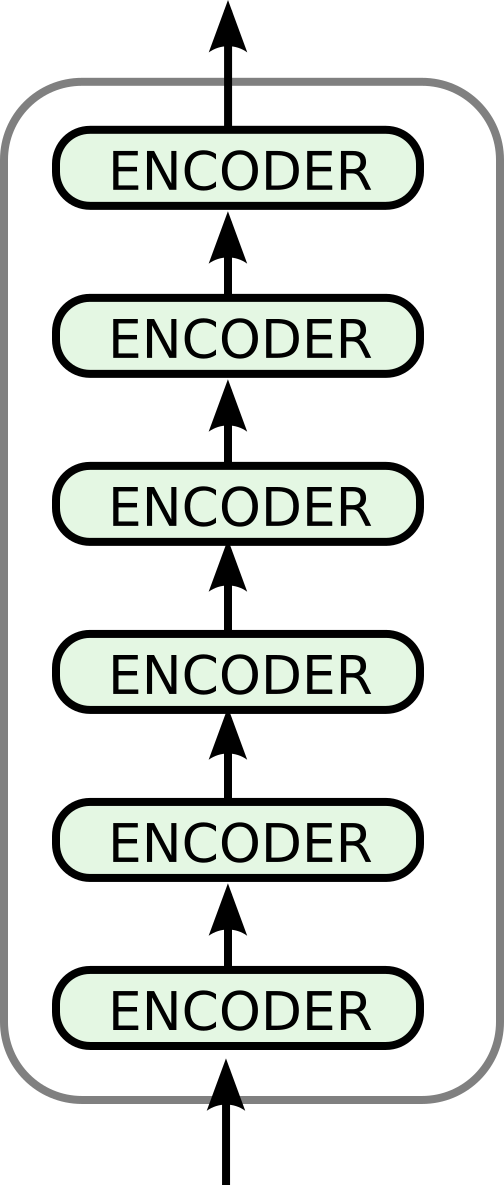
\includegraphics[angle=-90,scale=0.5]{BERT-Encoder.png}}}
	\end{equation}
\end{itemize}
\end{frame}

\begin{comment}
\begin{frame}
\frametitle{$N$ 个命题选 $K$ 个}
\begin{itemize}
\item \cc{At the porpositional level, attention 要用 weight matrix 记住各种命题之间的 相关性}
{At the propositional level, attention uses a \emp{weight matrix} to memorize the relatedness among propositions}

% \item 但逻辑 attention 和一般 attention 要求略有不同

% \item 不是「同类映射到同类」,而是要在 数量庞大的 logic rules 中 找到适用(applicable)的 rule

% \item 隐状态 $s_t$ 代表 ``search state'',注意力 的目的是 \emp{选择} $s_t$ 所需要的那些命题,交给 解码器

% \item 注意: 逻辑 attention 从 $M$ 个命题中 选择 $N$ 个命题,$M > N$. 这是 inductive bias. \ 而 symmetric NN 的做法,只是要求 $M$ 个命题 的 \emp{置换不变性},所以它浪费了资源在很多 ``don't care'' 的命题上

% \item 换句话说,attention 或者可以加强 sym NN 的效率,甚至取代 sym NN

% \item \cc{例如,假设 $q$ 是被关注的逻辑命题,$p_1, p_2, .... $ 是一些可能相关的命题,$\bowtie$ 表示 matching by attention,我们希望输出它们的关联性:}
% {Suppose $q$ is the proposition under focus, $p_1, p_2, ....$ are some possibly relevant propositions, $\bowtie$ denotes matching by attention, we want to output their relatedness:}
%	\begin{equation}
%	q \bowtie \; \; p_1, p_2, ... \mapsto \mbox{related?}
%	\end{equation}
% \cc{但每个 case 需要 矩阵的一行 储存}
% {but each case takes one row of matrix for storage}

% \item \cc{这是一种 ``flat'' representation of cases}
% {This is a ``flat'' representation of cases}

% \item \cc{而如果我们企图使用 hierarchical 的方法处理,这个方向 会越来越变得像 deep learning, 还不如干脆使用 神经网络!}
% {If we try to use \emp{hierarchical} techniques to handle this, it becomes more and more like deep learning, we might as well just use a neural network!}

% \item \cc{换句话说: 直接使用 deep symmetric NN, 在 NN \emp{内部} 学习如何 选择 相关的命题}
% {In other words, use a deep symmetric NN, let it learn \emp{internally} how to select relevant propositions}

\item 我模仿 BERT 的优点(它将 RNN unfold 成 CNN,可以并行处理),从 $N$ 个命题中 预先选出 $N \choose K$ 组,每组尝试进行 推导:
\begin{equation}
\vcenter{\hbox{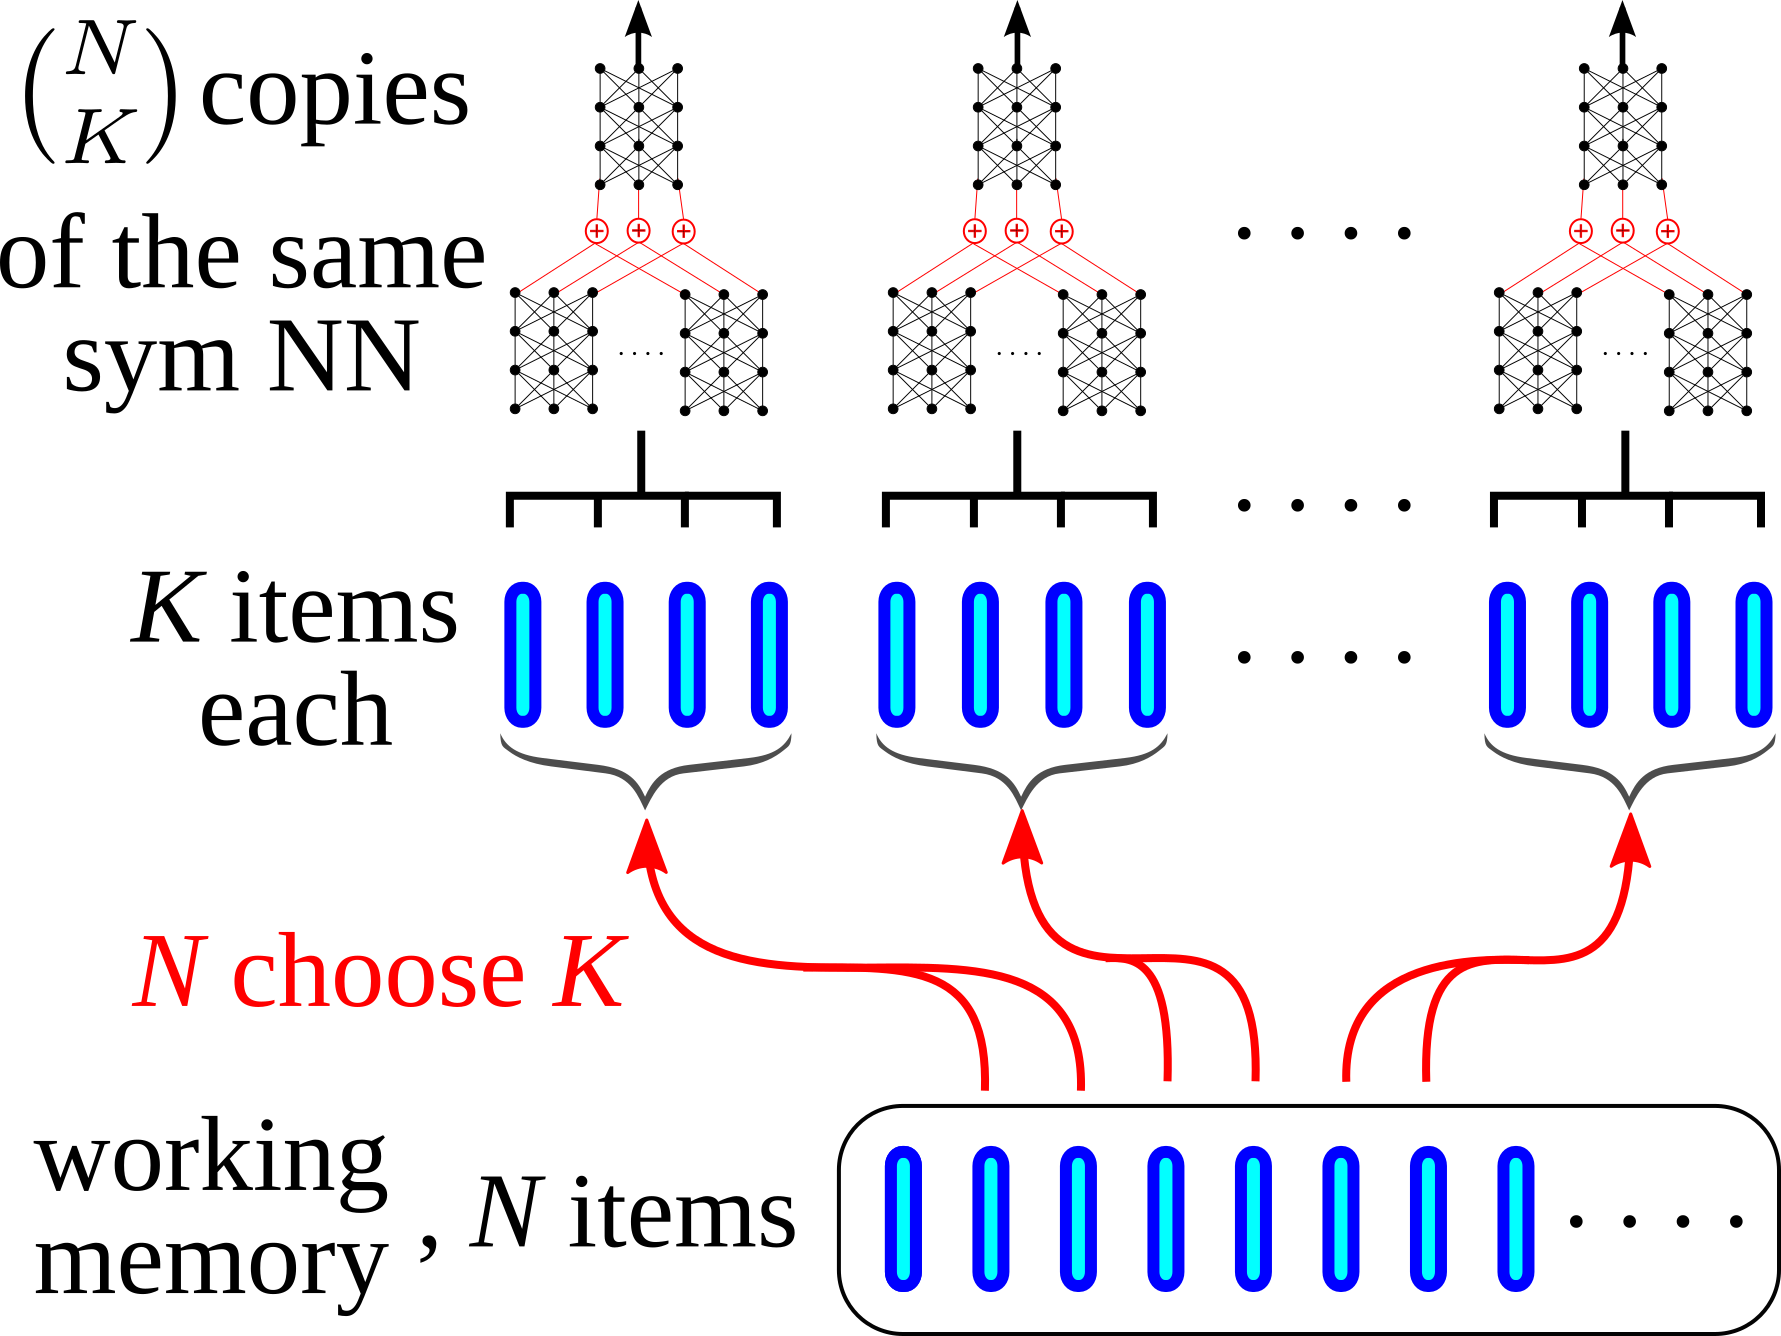
\includegraphics[scale=0.5]{N-choose-K.png}}}
\end{equation} 

\end{itemize}
\end{frame}
\end{comment}

\begin{frame}
\frametitle{Content-addressable long-term memory}
\begin{itemize}
	\item \cc{Content-addressable memory 的想法来自 Alex Graves \textit{et al} 的 Neural Turing Machine [2014]}
	{The content-addressable memory idea came from Alex Graves \textit{et al}'s Neural Turing Machine [2014]}

	\item \cc{以前 BERT 的隐状态 没有逻辑结构,我们不是很清楚它的内容是什么; 逻辑化之后,BERT 内部的命题可以储存在 \emp{长期记忆} 中:}
	{The original BERT's hidden state lacked a logical structure;  It was not clear what it contains exactly.  With logicalization, propositions inside BERT can be stored into a \emp{long-term memory}:}
	\begin{equation}
	\vcenter{\hbox{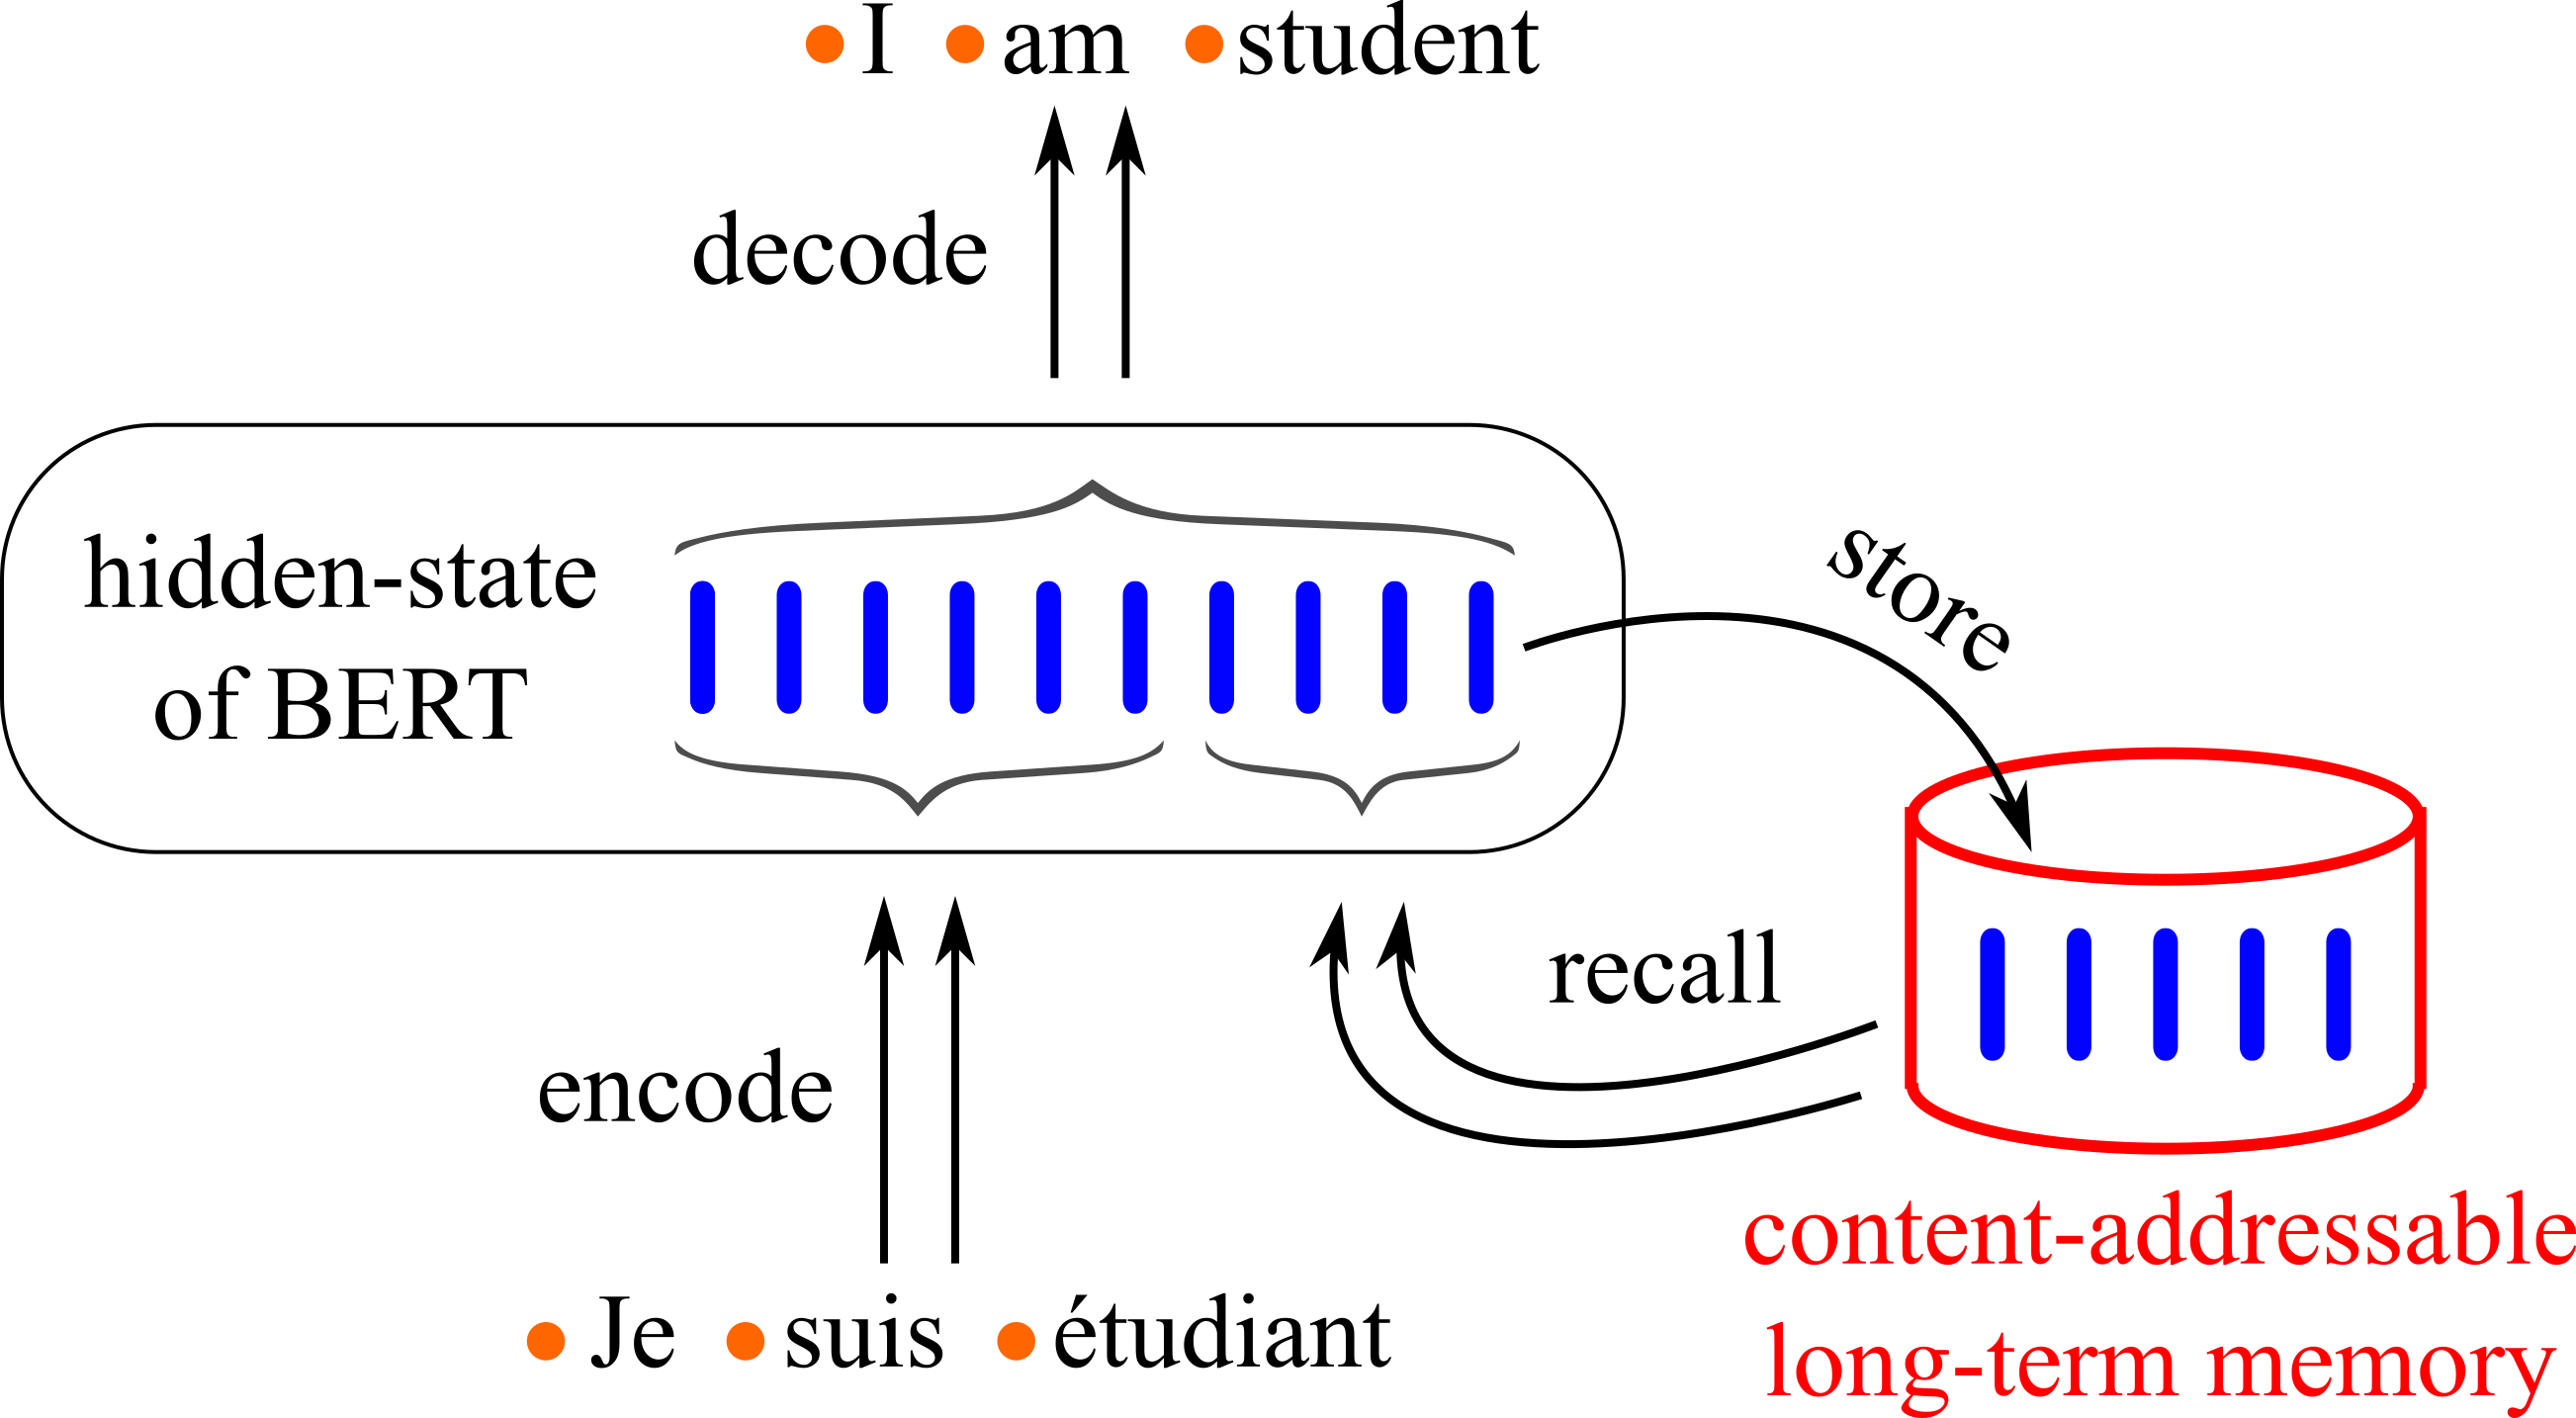
\includegraphics[scale=0.5]{long-term-memory.png}}}
	\end{equation}

	% \item 训练的方法,可以将所有 \NewSym{proposition.png} 存进 memory,如果对结论有帮助则加分,错则减分
	
	\item \cc{命名:}{Name:} \emp{K}nowledge-\emp{E}nhanced \emp{R}easoning with \emp{M}emorized \emp{It}ems

	\item \cc{这种系统 已非常接近 strong AI,而这是有赖 \emp{逻辑化} 才能做到的}
	{This is getting very close to strong AI, and depends crucially on logicalization}

 \end{itemize}
\nocite{Graves2014}
\end{frame}

\begin{frame}[plain]
\begin{itemize}
	\item \cc{例如:「太阳是热的」、「水向下流」是经常正确的命题}{Eg. ``The sun is hot'', ``Water flows downhill'' are facts that stay constant}

	\item \cc{
	但这些知识很多是 implicitly 存在於 rules (matrix weights) 之中}{
	But some of this knowledge is implicitly stored as rules (matrix weights)
	}
	
	\item \cc{
	也有些知识是 explicit 的,例如:「猫是哺乳类动物」、「吸烟可以致癌」}{
	Some knowledge is explicit, eg: ``cats are mammals'', ``smoking can cause cancer''
	}
	
	\item \cc{
	逻辑化理论提供一种 诠释 logic rules (weights) 的方法}{
	Logicalization provides a way to interpret logic rules (weights)
	}
	
	\item \cc{
	也可以将 weights 存进 content-addressable memory}{
	We can also store rules (weights) into content-addressable memory
	}
\end{itemize}
\end{frame}

\begin{frame}
\frametitle{\cc{对 逻辑主义 的质疑}
{Doubts about logicism}}
\begin{itemize}
	\item \cc{很多人怀疑: 人脑真的用 逻辑 思考吗?}
	{Many people question: Do our brains really use symbolic logic to think?}
	
	\item \cc{其实我们每句表达的 \emp{语言},都是逻辑形式的 (logical form)}
	{To say the least, all our languages are essentially in \emp{logical form}}

	\item \cc{直觉认为,人脑 构造一些 \emp{models},再从 model 中「读出」一些结论}
	{Our impression is that the brain constructs ``mental models'' of the world and ``reads off'' conclusions from such models}
	
	\item \cc{例如给定一个描述:「已婚妇人出轨,用刀刺死丈夫」}
	{Consider a description: ``Wife cheats on husband, stubs him with knife''}
	\begin{equation}
	\vcenter{\hbox{
\includegraphics[scale=1.0]{murder-scene.png}}}
	\end{equation}
	
	\item \cc{那么 妻子穿著什么衣服? 衣服什么颜色? 这些都是 \emp{臆想} 出来的细节,是不正确的}
	{What is she wearing? What color is her dress? Such details are \emp{imagined} and unwarranted}

	\item \cc{这个 model 可以有哪些细节? 答案是: 任何细节都不可以有,除非是 逻辑上蕴含的,或被 逻辑约束}
	{So what kind of details can our model have? The answer is: it cannot have ANY detail, except those entailed or constrainted by \emp{logic}}
	
	% \item 所以,其实所谓 ``model-based reasoning'' 并没有那么神奇,也并不一定正确,它的细节必需被 \emp{逻辑} 约束
	
	\item \cc{Model 本身可以是一些 抽象的逻辑命题 构成的,这也合理; 反而,一个有很多感官细节的 model 并不合理}
	{Models may be constructed from abstract logic propositions;  Models with a lot of sensory details are implausible}
	
	\item \cc{其实人脑可能 比我们想像中 更接近逻辑}
	{Perhaps the brain is much closer to formal logic than we'd thought}
\end{itemize}
\end{frame}


\frameinlbffalse
\begin{frame}
\frametitle{References}
\cc{欢迎提问和讨论}{Questions, comments welcome} \smiley \\ \vspace*{0.4cm}
\printbibliography
\end{frame}

\end{document} 